\documentclass[10pt, conference]{IEEEtran}

% ------------- Packages Used --------------------------------------------------
% They help us to produce a better looking document ;-)
% ------------------------------------------------------------------------------

% Comment the following line before compiling the final version
%\synctex

\usepackage{url}
\usepackage{listings}
\usepackage{color}
\usepackage{balance}
\usepackage{graphicx}
\usepackage[justification=centering]{caption}
\definecolor{dkgreen}{rgb}{0,0.6,0}
\definecolor{gray}{rgb}{0.5,0.5,0.5}
\definecolor{mauve}{rgb}{0.58,0,0.82}
\usepackage{multirow}
\usepackage{booktabs}
\usepackage{amsmath}
%\usepackage{mathtools}

\lstset{frame=tb,
  language=Java,
  aboveskip=3mm,
  belowskip=3mm,
  showstringspaces=false,
  columns=flexible,
  basicstyle={\small\ttfamily},
  numbers=none,
  numberstyle=\tiny\color{gray},
  keywordstyle=\color{blue},
  commentstyle=\color{dkgreen},
  stringstyle=\color{mauve},
  breaklines=true,
  breakatwhitespace=true,
  tabsize=3
}

\usepackage{multirow}
\usepackage{balance}
\usepackage{graphicx}
\usepackage{alltt}
\usepackage{relsize}
%\usepackage{xspace}
\usepackage{booktabs}
\usepackage{array}
\usepackage{amsmath}
%\usepackage{multirow}
%\usepackage{array}
\usepackage{verbatim}

%\usepackage{subfigure}
\usepackage[tight,footnotesize]{subfigure}

%\usepackage{capt-of}
%\usepackage{pifont}
\usepackage{amsfonts}
\usepackage{amssymb}
%\usepackage[latin1]{inputenc}
%\usepackage{times}
%\usepackage{colortbl}
\usepackage{boxedminipage}
\usepackage{float}
\usepackage{cite}
\usepackage{fancyvrb}
\usepackage[dvipsnames]{xcolor}
%\usepackage{hyperref}
\usepackage{balance}
\usepackage{url}
\usepackage{fancybox}%for \hypobox
\usepackage{listings}
\usepackage{array}
\usepackage{multicol}
%\usepackage{chngpage}
%\usepackage{booktabs}

%\usepackage{textcomp}
%\usepackage{latexsym}
%\usepackage{amssymb}
%\usepackage{stmaryrd}
%\usepackage{euscript}
%\usepackage{wasysym}
%\usepackage{pifont}
%\usepackage{manfnt}
%\usepackage{undertilde}
%\usepackage{ifsym}
%\usepackage{tipa}
%\usepackage{txfonts}
%\usepackage{skak}
%\usepackage{skull}
%\usepackage{eurosym}
%\usepackage{yfonts}
%\usepackage{mathdots}
%\usepackage{trsym}
%\usepackage{upgreek}
%\usepackage{chemarr}
%\usepackage{accents}
%\usepackage{nicefrac}
%\usepackage{bm}


%\usepackage{pdfsync}

%   ACM Style
%\usepackage{lcsect}
% ------------------------------------------------------------------------------






% ------------ Color Definitions -----------------------------------------------
% Whatever colors we need
% ------------------------------------------------------------------------------
\definecolor{mygray}{rgb}{0.7,0.7,0.7}
% ------------------------------------------------------------------------------






% ---------- Special commands for annotating the paper's text ------------------
\let\mymarginpar\marginparm
\marginparwidth=1cm
\marginparsep=5pt
\newcommand{\todo}[1]{\textcolor{red}{\textbf{[[#1]]}}}
\def\TODO#1{\noindent\colorbox{yellow}{\bf \textcolor{red}{TODO: #1}}}
\newcommand{\hint}[1]{\textcolor{blue}{\textbf{#1}}}
\def\fig#1{Figure~\ref{#1}}
\def\tab#1{Table~\ref{#1}}
\def\eqn#1{Equation~\ref{#1}}
\def\sec#1{Section~\ref{#1}}

\pagenumbering{arabic}
\newcommand{\reviewer}[1]{\textcolor{DeepPink1}{{\it [Reviewer says: #1]}}}
\newcommand{\mei}[1]{\textcolor{red}{{\it [Mei says: #1]}}}
\newcommand{\hammam}[1]{\textcolor{red}{{\it [Hammam says: #1]}}}
\newcommand{\ian}[1]{\textcolor{blue}{{\it [Ian says: #1]}}}
\newcommand{\nic}[1]{\textcolor{WildStrawberry}{{\it [Nico says: #1]}}}
\newcommand{\ahmed}[1]{\textcolor{green}{{\it [Ahmed says: #1]}}}
\newcommand{\myfoot}[1]{\footnote{\scriptsize #1}}
\newcommand{\myurl}[1]{\myfoot{\url{#1}}}
\newcommand{\Ra}{{$\Rightarrow$}}
\newcommand{\ra}{{$\rightarrow$}}
\newcommand{\La}{{$\Leftarrow$}}
\newcommand{\la}{{$\leftarrow$}}
\newcommand{\lra}{{$\leftrightarrow$}}
\newcommand{\LRa}{{$\Leftrightarrow$}}
%\newcommand{\todo}{\bram{todo}}

\newenvironment{myindentpar}[1]%
{\begin{list}{}%
         {\setlength{\leftmargin}{#1}}%
         \item[]%
}
{\end{list}}

% \AtBeginDocument{%
%    \renewcommand{\figurename}{Figure}%
%    \newcommand{\subfigureautorefname}{\figureautorefname}%for using subfig
% %   \renewcommand{\tablename}{TABLE}%
%    \renewcommand{\tablename}{Table}%
%    \renewcommand{\subsectionautorefname}{Section}%
%    \renewcommand{\sectionautorefname}{Section}%
% }

% Hypothesis box
% ------------------------------------------------------------------------------
\newcommand{\hypobox}[1]{\begin{center}%
        \noindent\thicklines\setlength{\fboxsep}{6pt}%
        \cornersize{0}\Ovalbox{\begin{minipage}{3.2in}%
        \vspace{-0.2cm}
        \textit{#1}
        \vspace{-0.2cm}
        \end{minipage}} \end{center}}
% ------------------------------------------------------------------------------




% ------------------------- SYMBOLS OF SELF NAMES OFTEN USED -------------------
\newcommand{\APACHE}{{\small APACHE}\xspace}
\newcommand{\BUGZILLA}{{\small BUGZILLA}\xspace}
\newcommand{\ECLIPSE}{{\small ECLIPSE}\xspace}
\newcommand{\ASPECTJ}{{\small ASPECTJ}\xspace}
\newcommand{\JDT}{{\small JDT}\xspace}
\newcommand{\GNU}{{\small GNU}\xspace}
\newcommand{\MOZILLA}{{\small MOZILLA}\xspace}
\newcommand{\THUNDERBIRD}{{\small THUNDERBIRD}\xspace}
\newcommand{\JAVA}{{\small Java}\xspace}
\newcommand{\GNOME}{{\small GNOME}\xspace}
\newcommand{\PG}{{\small PostgreSQL}\xspace}
\newcommand{\SIM}{{\small SimScan}\xspace}

% Anything else, e.g., \NAME{MICROSOFT}
\newcommand{\NAME}[1]{{\small #1}\xspace}
% ------------------------------------------------------------------------------




% ----------------------- Computer Science lol ---------------------------------
% Variable, function, and program names
% ------------------------------------------------------------------------------
\newcommand{\smalltt}[1]{\ifmmode{\mbox{\smaller\texttt{#1}}}\else{\smaller\tt #1}\fi}
\newcommand{\code}[1]{\smalltt{#1}}
\newcommand{\var}[1]{\code{#1}}
\newcommand{\func}[1]{\code{#1}}
\newcommand{\proc}[1]{\code{#1}}
\newcommand{\prog}[1]{\code{#1}}
\newcommand{\type}[1]{\code{#1}}
\newcommand{\progpt}[1]{\code{#1}}

\newcommand{\mypar}[1]{\vspace{.1cm}\noindent \textbf{#1}}
\newcommand{\myxpar}[1]{\vspace{.1cm}\noindent \textbf{#1}\newline}
% ------------------------------------------------------------------------------





% ----------- Things to remember -----------------------------------------------
\newenvironment{mynote}%
{ \medskip
  \noindent
  \let\emph=\textbf
  \begin{boxedminipage}{\columnwidth}\em}%
{ \end{boxedminipage}}
% ------------------------------------------------------------------------------






% -------------------- Use bars ------------------------------------------------
% These macros are for advanced presentation of results by shaded bars only!
% © Tom Zimmermann, 2008
% ------------------------------------------------------------------------------
\newdimen\qdx
\newdimen\qda
\newdimen\qdb
\def\rrrr#1#2#3#4{\newdimen\qd\qd=#4 % length of bar for 1.0
\qdx=\qd\multiply\qdx by 5\divide\qdx by 4
\qda=\qd
\qdb=\qd
\multiply\qda by #1\divide\qda by #3\multiply\qdb by #2\divide\qdb by #3\advance\qdb by -\qda
    \leavevmode\hbox to \qdx{\hfil\vbox{%
    \hbox{\vrule\vbox{\hrule\hbox to 1\qd
            {\vrule depth0pt height0.7ex width \qda\color{mygray}%
 \vrule depth0pt height0.7ex width \qdb\hfill}\hrule}\vrule}
    }\hfil}}
\def\rrr#1#2#3{\rrrr{#1}{#2}{#3}{0.8cm}}
% -------------------------------------------------------------------------






% ------------ Graphics Hacks --------------------------------------------------
% Use these settings if Figures tend to get their one separate pages
% ------------------------------------------------------------------------------
% \renewcommand{\topfraction}{0.85}
% \renewcommand{\textfraction}{0.1}
% \renewcommand{\floatpagefraction}{0.75}
% ------------------------------------------------------------------------------





% ------------------ Biblio Hack -----------------------------------------------
% Use these settings if the References take too much space
% ------------------------------------------------------------------------------
\let\oldthebibliography=\thebibliography
  \let\endoldthebibliography=\endthebibliography
  \renewenvironment{thebibliography}[1]{%
%       \vspace{-0.3cm}
    \begin{oldthebibliography}{#1}%
%       \vspace{-0.2cm}
       \setlength{\parskip}{0ex}%
       \setlength{\itemsep}{0ex}%
%       \bibfont
  }%
  {%
    \end{oldthebibliography}%
  }
% ------------------------------------------------------------------------------





% -------------- Floats Redefined ----------------------------------------------
% Use these settings to change the whitespace between floats and text
% ------------------------------------------------------------------------------

% \setlength\dblfloatsep{1pt}
% \setlength\floatsep{1pt}
% \setlength\textfloatsep{5pt}
% \setlength\dbltextfloatsep{5pt}

% \renewcommand\floatpagefraction{.9}
% \renewcommand\topfraction{.9}
% \renewcommand\bottomfraction{.9}
% \renewcommand\textfraction{.1}
% \setcounter{totalnumber}{50}
% \setcounter{topnumber}{50}
% \setcounter{bottomnumber}{50}
% ------------------------------------------------------------------------------


\newcommand{\specialcell}[2][c]{%
        \begin{tabular}[#1]{@{}c@{}}#2\end{tabular}}


\usepackage{subfigure}
%\usepackage{subfig}
\usepackage{balance}
\usepackage{balance}
\usepackage{amssymb,amsmath}
\usepackage{wrapfig}
\usepackage{multirow}
\usepackage{graphicx}
\usepackage{algorithm}
\usepackage{algorithmic}
\usepackage{times}
\usepackage{cite}
\usepackage{fancybox}
\usepackage{color}
\usepackage{array}
\usepackage{subfigure}
\usepackage{balance}
\usepackage{epstopdf}
\usepackage{array}
%\usepackage{subfig}
%\usepackage{xspace}
\def\UrlBreaks{\do\/\do-} %to break the urls, all in one line



\newcommand{\conclusionbox}[1]{%
	\vspace{2mm}
	\framebox[0.45\textwidth][c]{%
		\parbox[b]{0.42\textwidth}{%
			{\it #1}
		}
	}
	\vspace{2mm}
}

\newcommand{\emad}[1]{\textcolor{red}{{\it [Emad says: #1]}}}
%\newcommand{\todo}[1]{\colorbox{yellow}{\textbf{[#1]}}}


\newcommand{\rqi}{\textbf{}}
\newcommand{\rqii}{\textbf{}}
\newcommand{\rqiii}{\textbf{}}

\begin{document}
\title{Studying the Discrepancy between Performance Testing Results from Virtual and Physical Environments}

\author{\IEEEauthorblockN{Muhammad Moiz Arif, Weiyi Shang, Emad Shihab}

\IEEEauthorblockA{Department of Computer Science and Software Engineering\\Concordia University,
Montreal, Canada\\
\url{{mo_ari,shang,eshihab}@encs.concordia.ca}}}

\maketitle
\thispagestyle{plain}
\pagestyle{plain}

\begin{abstract}
Performance plays an indispensable role for software reliability. 
%The unreliability of software systems in the field is often caused by performance issues than functional bugs. 
Performance tests are typically conducted in order to ensure the performance of software systems. Such performance tests often consume large amounts of computing resources, such as long running time in the performance testing environments. Making it worse, the ever evolving field environment requires frequently updating the performance testing environment. In practice, virtual machines (VMs) are widely exploited to provide flexible and less costly environments for performance tests. However, the use of VMs may introduce extra overheads (e.g., a higher than expected memory utilization) to the testing environment, leading to un-realistic performance testing results. Yet, to the best of our knowledge, little research has studied such overhead in the context of performance testing activities, nor has investigated the impact on performance testing results. 
		
In this paper, we perform a case study on two open source systems, i.e., Dell DVD Store and CloudStore, to evaluate the discrepancy between the performance testing results from virtual and physical environments. We conduct the same performance tests in both virtual and physical environments. In order to evaluate the discrepancy, we compare the performance testing results based on the three aspects that are typically examined for performance testing results: 1) individual performance metric, 2) relationship among performance metrics and 3) performance models that are build from the performance metrics. Our results illustrate the discrepancy between performance testing results from virtual and physical environments. In particular, individual performance metrics from virtual and physical environments do not share the same shape of distribution. The correlations among performance metrics in virtual environment are different from the correlations in physical environment. Finally, the statistical models that are built based on the performance counters from virtual environment are different from the models that are build from the physical environment. Normalizing performance metrics based on deviance may reduced such discrepancy. Practitioners should be aware of such discrepancy and may leverage normalization techniques when analyzing performance testing results from virtual environments.


		
		
	%	activities, including performance modeling and performance regression detection. The two activities are conducted in both environments that consists of physical machines or VMs. We observed that the comparison between the virtual and physical environments is not straight forward. We also observed that the performance of our subject systems between two environments is not identical.
		
	%	\textcolor{red}{(insert implications)}
	
%	\textit{Keywords--Performance engineering; Performance testing; Performance modeling; Performance analysis}	
	\end{abstract}
	

\section{Introduction}
\label{sec:introduction}
% -*- root: cuthesis_masters.tex -*-  

%At the core of any software system is the software team who develop it...

\section{Introduction}
%Cloud computing has eliminated the need for hardware decisions. It is now a significant part of the IT industry incorporating not only the leading names like \textit{Facebook, Amazon, Google} etc but also small-scaled business ventures that are migrating on to a cloud based environment. According to a survey \textit{'survey'}, up to 70\% of the companies are moving from conventional physical data servers? to cloud based servers. The primary concerns when migrating are, usually, costs, availability performance etc of the system. 
%Software Performance Engineering(SPE) incorporates all the software engineering activities carried out during the project's lifecycle required to meet the software's performance requirements.
%These performance requirements ensure that the user requests are served are in a timely manner and the software's response time does not degrade with the increase in workload i.e. users. In the midst of todays large-scale software systems, (e.g.Amazon and Google's Gmail), SPE plays a vital role as most of the failures are associated with performance than with feature bugs. A second's downtime of amazon.com would cost millions of dollars. One of the recent examples in this regard was the roll-out failure of healthcare.gov. Another example was the crash of Facebook which caused NASDAQ a high monetary misfortune. 
%To avoid performance failures, software performance engineers use performance testing. The tests are used to exercise the subject system which is under test. To exercise this system, it is subjected to different workloads. These tests are designed to uncover performance bottlenecks or a test objective like maximum operational capacity. 
%The goal of performance testing is to test how the system responds are realistic workloads. Therefore performance test are composted of test workload and configuration of SUT which represents a field like environment. 
%The goal of this study is to compare the performance of a SUT in heterogeneous environments. Due to lack of resources and constant requirement of evolution of the testing environment practitioners often rely on testing done in virtual environments. However, the road that leads to the reliability of performance activities done in virtual environments still remains undiscovered. 
%Performance is a big deal
Software performance assurance activities play a vital role in the development of large software systems. These activities ensure that the software meets the desired performance requirements~\cite{futureofspe}. Often however, failures in large software systems are due to performance issues rather than functional bugs~\cite{tailatscale, foo2010mining}. Such failures lead to the eventual decline in quality of the system with reputational and monetary consequences~\cite{costofdowntime}. For instance, Amazon estimates that a one-second page-load slowdown can cost up to \$1.6 billion~\cite{amazononesec}. 

%The impact from performance issues on system reliability would also lead to serious reputational issues.

%an interruption in the Amazon Web Service lead to the disruption of Quora, Reddit, Foursquare and numerous other web sites~\cite{amazondown}. 

%In the software ecosystem, performance assurance activities play a vital role \cite{Shang:2015:ADP:2668930.2688052}. In essence, these activities ensure a consistent software functionality. The trend of dedicating a large chunk of costs, in some cases even exceeding the cost of development \cite{bertolino2007software} to such performance assurance activities is now not unusual. In fact, most of the problems in the field are due to performance related issues \cite{foo2010mining} . A failure here would not only include an eventual decline in the quality of the software but also monetary and temporal losses. That is why companies like \textit{Facebook, Amazon and Google} are committed to achieve excellence in this regard. \cite{jackson2010performance}

% Practitioners use performance tests
In order to mitigate performance issues and ensure software reliability, practitioners often conduct performance tests~\cite{futureofspe}. Performance tests apply a workload (e.g., mimicking users' behavior in the field) on the software system~\cite{ranjanbook,Syer2016}, and monitor performance metrics, such as CPU usage, that are generated based on the tests. Practitioners use such metrics to gauge the performance of the software system and identify potential performance issues (such as memory leaks~\cite{markicsm2013} and throughput bottlenecks~\cite{5635038}).

%Performance tests are subjected to highlight system's performance which are congruent to a field-like load~\cite{Shang:2015:ADP:2668930.2688052, Syer2016}. For example, to investigate the performance bottlenecks, the maximum throughput of the system~\cite{syer2014maintenance} or other the non-functional performance requirements.

%The objective behind performance regression testing is to identify if there exists a lapse in performance for the newer version of the software compared to the previous versions. The system is tested by applying a fixed load which is congruent to a field-like load \cite{Shang:2015:ADP:2668930.2688052} \cite{foo2010mining} \cite{5306331}. The performance analysts then look for deviations between metrics values compared to the earlier versions. Examples of factors causing performance lapse may be because of high CPU utilization or a memory leak. \cite{5306331}. As there are no benchmarks for measuring the software performance cross environments, and with little or no time dedicated to performance assurance activities practitioners often find it hard to test and analyze the results of regression testing.

%The need for performance testing environments to advance and evolve is continually augmenting and so is the cost associated with the environment~\cite{stpmag, bertolino2007software}. 

%One of challenges practitioners face is the lack of available resources for performance testing. For instance

%People perform things on virtual environments
Since performance tests are often performed on large-scale software systems, the performance tests often require many resources~\cite{ranjanbook}. Moreover, performance tests often need to run for a long period of time in order to build statistical confidence on the results~\cite{ranjanbook}. In addition, such testing environment needs to be easily configurable such that a specific environment can be mimicked, reducing false performance issues. For example, issues that are related to the environment. Therefore, to address such challenges, virtual environments (i.e., VMs) are often leveraged for performance testing~\cite{whyvirtualisbetter, vmwarehighcost, whyvirtualisbetter}. The flexibility of virtual environments enables practitioners to easily prepare, customize, use and update performance testing environments in an efficient manner.

%Making it worse, the diversified and ever-changing users' behaviour forces the testing environments to be frequently customized and updated~\cite{Syer2016}.

%More importantly, performance testing is often last stage of the software development lifecycle which forces the managers to dedicate a minimal time for performance testing which can even span out to days. That's why practitioners prefer testing the system in a virtual environment~\cite{whyvirtualisbetter, vmwarehighcost}. The choice of running the performance assurance activities in a virtual environment is also based on the complexity of the large scale software systems. This enforces a virtual set up of the environment which saves resources and is easier to set up according to the desired needs~\cite{VMWarePowerCLIBlog, seetharaman2006test}. 

% No one looked at the applicability across platforms
%However, a major question that lingers is that \textbf{are performance tests executed in a virtual environment representative of what happens in the physical environment?}. This question is particularly important since 1) virtual environments are highly leveraged in practice~\cite{Nguyen:2012:ADP:2188286.2188344,xiong2013vperfguard} and 2) prior work has shown that using virtual machines imposes a hidden overhead that is rarely considered~\cite{menon2005diagnosing}, impacting the reliability of performance test results performed in virtual environments. 

Prior studies show that virtual environments are widely exploited in practice~\cite{Cito:2015:MCA:2786805.2786826,Nguyen:2012:ADP:2188286.2188344,xiong2013vperfguard}. Studies have investigated the overhead that is associated with virtual environments~\cite{menon2005diagnosing}. Such overheads may not impose effect on the results of performance tests carried out in physical and virtual environments. For example, if the performance (e.g., throughput) of the system follows the same trend (or distribution) in physical and virtual environments, such overhead would not significantly impact on the practitioners who examine the performance testing results. To the best of our knowledge, the discrepancy between performance testing results in virtual and physical environments has never been studied. Exploring, identifying and minimizing such discrepancy will help practitioners and researchers understand and leverage performance testing results from virtual and physical environments. Without knowing if there exists a discrepancy between the performance testing results from the two environments practitioners cannot rely on the performance assurance activities carried out in the virtual environment or vice versa. Once the discrepancy is identified, the performance results could be evaluated more accurately.



%Whether virtual environments are applicable in performance assurance activities or if they can be relied to behave equivalent to the physical servers still remains questionable. There have been limited instances of diagnosis of performance overheads~\cite{menon2005diagnosing} in the domain of performance testing however no concrete conclusions have been drawn yet. 

%The goal of our study is evaluating the discrepancy between the performance testing results from virtual and physical environments. 
%Additionally, we investigated if the performane tests done in virtual environments are repeatable or not. 
%Additionally, if they do not belong to the same population, then how impactful and effective are the prevalent discrepancies for a model-based regression testing approach.    


%what we do
In this thesis, we perform a study on two open-source systems, DS2~\cite{delldvd} and CloudStore~\cite{cloudstore}, where performance tests are conducted on virtual and physical environments. Our study focuses on the discrepancy between the two environments, the impact of discrepancy on performance testing results and highlights potential opportunities to minimize the discrepancy. In particular, we compare performance testing results from virtual and physical environments based on the three widely examined aspects, i.e., individual performance metric, the relationship between the performance metrics and models that predict performance. 
%by running performance tests in both virtual and physical environments. We compare the performance test results that are generated from both the environments. In particular, we compare the performance testing results by 1) examining individual performance metric, 2) examining relationship among performance metrics and 3) building statistical models using performance metrics. 

%what we find


%Our findings highlight the need of awareness of the discrepancy between performance testing results in virtual and physical environments, and the need to research efforts on investigating how to improve the use of both virtual and physical environments to ensure system reliability.

%We leverage a heatmap to visualize the changes in correlations among performance metrics and the system load metric.

% cannot apply on the performance metrics collected from another environments (with high prediction error), even after normalizing the performance metrics.


%In particular, we first compare the performance metrics values and distributions. We then investigate the correlation of performance counters to the generated load. Finally, we build statistical models to help us reach conclusions. 
%We observed that majority of the performance counters do not belong to the same family of distribution. We also observed that the metric that are highly correlated with the load are not the same across both our subject systems.
%We concluded that due to the discrepancies present in the virtual environment, we can not rely on performance evaluated in the virtual environment as is. We then apply scaling techniques to the metrics generated in the virtual environment to build linear regression models. We concluded that the performance metrics in the virtual environment are not identical copies of the metrics in the physical environment. 


% to determine and compare the distributions. This is achieved by comparing plots and finding correlation between the metrics cross-environments. We use generalized linear regression models, as used in the performance assurance activities \cite{Shang:2015:ADP:2668930.2688052}, to determine the extent of the comparison between metrics. If the metrics are transferable between the environments, we should expect to see a low percentage error. We chose to build our regression models based on multiple performance metrics to see the effect of the clustered performance metrics. 

%We diffuse our findings by answering the following research questions:

%\begin{description}
%	\item[$\bullet$] RQ1: Do performance metrics from physical and virtual environments belong to the same population?
%	\item[$\bullet$] RQ2: Is the metric correlation with load same cross-environments?
%	\item[$\bullet$] RQ3: Do performance metrics from different environments impact performance modeling?

%\end{description}

\section{Research Hypothesis}
Prior research and our industrial experience lead us to an investigation based on the following hypothesis:
%	\fbox{%
%		\parbox{\textwidth}{%
%			\textit{
%			For large-scale software systems, performance assurance activities are carried primarily in virtual environments. There is little research regarding the reliability of testing in a different environment compared to physical. We hypothesize that for software testing activities there exists a discrepancy between physical and virtual environments. We believe that the approaches used so far do not scale well. 
%			Furthermore, we believe practitioners should be aware of such existing discrepancies when analyzing software performance in a foreign environment.
%				   }
%		}%
%	}
	
\begin{framed}
		\textit{For large-scale software systems, performance assurance activities are carried primarily in virtual environments. There is little research regarding the reliability of testing in a different environment compared to physical. We hypothesize that for software testing activities there exists a discrepancy between physical and virtual environments. We believe that the approaches used so far do not scale well.} 
		\par 	
		\textit{Furthermore, we believe practitioners should be aware of such existing discrepancies when analyzing software performance in a foreign environment.}
\end{framed}



\section{Thesis Overview}

%The rest of the paper is organized as follows. Section~\ref{sec:related} presents the background and related work. Section~\ref{sec:case} presents the case study setup. Section~\ref{sec:results} presents the results of our cases study, followed by a discussion of our results in Section~\ref{sec:discussion}. Section~\ref{sec:threats} discusses the threats to validity of our findings. Finally, Section~\ref{sec:conclusion} concludes this paper.

\textbf{Chapter 2: Literature Review:} In this chapter, we discuss the related work that has discussed performance assurance activities carried out in virtual environments and the associated overhead caused by it. The chapter is divided in two parts:

	\textbf{Part I:} Addresses the methodologies that are used to detect performance anomalies. We present the work sub divided into three categories: individual performance metrics, relationship among performance metrics, statistical modeling based on performance metrics.   
	
    \textbf{Part II:} Addresses the work that points to the overheads present in virtual environments. We present the state-of-the-art approaches used to detect performance anomalies and how such approaches helps us in detection of overheads. The chapter wraps up by comparing the current limitations and our work in the field of performance engineering.

From the literature review, we deduced that a lot of work has been affiliated to the generation of performance alarms and the detection of performance issues however little work has highlighted the reliability of testing done in virtual environments.
\\

\noindent\textbf{Chapter 3: Testing For the Ubiety of Discrepancy:} In this chapter, we perform case studies on two open source subject systems. We generate the performance metrics by applying realistic and varying workloads in identically set up physical and virtual environments. Followed up data cleansing and removing any reasonable outliers present in our data. Next, we analyze the performance metrics in three possible ways: individually, as a collection, and as an input to statistical models. 
\\

\noindent\textbf{Chapter 4: Studying the impact of modifying the virtual environment}
Furthermore, we elaborate and solidify the conclusion drawn by discussing possibilities as how the use of virtual environments may effect our results: by changing the type of the virtual machine, by modifying the allocated resources and testing the repeatability(hence the stability) of our chosen virtual environment.
Lastly, we discuss the threats to validity for this thesis.
\\


\section{Thesis Contributions}

The major contributions of thesis are as follows:

\begin{itemize}
	\item An extensive review of the state of the art in software performance activities carried out in virtual environments. Such a review is necessary for the practitioners to be aware of the hiccups associated to software performance in virtual environments.
	
	\item We conclude performance metrics have different shapes of distributions and trends in virtual environments compared to physical environments. There are large differences in correlations among performance metrics measured in virtual and physical environments.
	\item We highlight statistical models using performance metrics from virtual environments do not apply to physical environments (i.e., produce high prediction error) and vice versa.
	\item  We examined the feasibility of using normalizations to help alleviate the discrepancy between performance metrics. We find that in some cases, normalizing performance metrics based on deviance may reduce the prediction error when using performance metrics collected from one environment and applying it on another. 
	\item We demonstrate that practitioners cannot assume that their performance tests that are observed on one environment will necessarily apply to another environment. The overhead from virtual environments does not only impact the scale of the performance metrics, but also impacts the relationship among performance metrics. On the other hand, we find that practitioners who leverage both, virtual and physical environments, may be able to reduce the discrepancy that may arise due to the environment (i.e., virtual vs. physical) by applying normalization techniques.
\end{itemize}

\section{Related Work}
\label{sec:related_work}
The work that is most related to the paper can be categorized into two main areas: 1) analyzing performance metrics from performance testing, using individual performance metrics, relationship among performance metrics, and statistical modelling based on performance metrics, and 2) analysis of VM overhead. Here, we discuss the state-of-the-art and how our work relates to prior work.

\subsection{Analyzing performance metrics from performance testing} 

\noindent \textbf{Individual performance metrics}

Nguyen \textit{et al$.$}~\cite{Nguyen:2012:ADP:2188286.2188344} introduce the concept of using control charts~\cite{shewhart1931economic} in order to detect performance regression. Control charts use a predefined threshold to detect performance anomalies. However control charts assume that the output follows a uni-model distribution which may be an inappropriate assumption for performance. Nguyen \textit{ et al$.$} propose an approach to normalize performance metrics between heterogeneous environments in order to build robust control charts. %However, the experiments are only carried out on the virtual machines in contrast to our approach.

Malik \emph{et al$.$}~\cite{Malik:2010:ACL:1955601.1955936, haroon} propose approaches that cluster performance metrics using Principal Component Analysis (PCA). Each component generated by PCA is mapped to performance metrics by a weight value. The weight value measures how much a metric contributes to the component. For every performance metric, a comparison is performed on the weight value of each component to detect performance regressions.

Heger \emph{et al$.$}~\cite{DBLP:conf/wosp/HegerHF13} present an approach that uses software development history and unit tests to diagnose the root cause of performance regressions. In the first step of their approach, they leverage Analysis of Variance (ANOVA) to compare the response time of the system to detect performance regressions. Similarly, Jiang \emph{et al$.$}~\cite{jackicsm2009} extract response time from system logs. Instead of conducting statistical tests, Jiang \emph{et al$.$} visualize the trend of response time during performance tests, in order to identify performance issues.


%\emad{how does this compare to our work?}
%

%The ad hoc approach may fail to detect performance regressions if the target counters do not capture the performance regressions. Moreover, such ad hoc analysis does not detect the change of relationships between counters, such as the relationship between I/O and CPU.


\noindent \textbf{Relationship among performance metrics}

Malik \emph{et al$.$}~\cite{5635038} leverage Spearman's rank correlation to capture the relationship among performance metrics. The deviance of correlation is calculated in order to pinpoint which subsystem should take responsibility of performance deviation.

Foo\emph{ et al$.$}~\cite{foo2010mining} propose an approach that leverages association rules in order to address the limitations of manually detecting performance regression in large scale software systems. Association rules capture the historical relationship among performance metrics and generate rules based on the results of prior performance tests. Deviation in the association rules are considered signs of performance regressions.

Jiang \emph{et al$.$}~\cite{5270324} use normalized mutual information as a similarity measure to cluster correlated performance metrics. Since metrics in one cluster are highly correlated, the uncertainty among metrics in the cluster should be low. Jiang \emph{et al$.$} leverage entropy from information theory to monitor the uncertainty of each cluster. A significant change in the entropy is considered as a sign of a performance fault. %During the evaluation of the approach, the authors were able to detect 77\% of the injected faults and the faulty subsystems, without having any false positives.

%Our approach also considers the correlations between performance counters by using regression models. However, our approach first aims to group performance counters into test aspects and focuses on detecting performance regressions instead of faults.


%\emad{how does this compare}


%Malik\textit{ et al.}~\cite{haroon} derive performance signatures based on both supervised and unsupervised learning to detect performance anomalies. They use Principal Component Analysis as their unsupervised learning technique if the past tests are not marked pass or fail. PCA is used to to examine the relationships between different performance metrics.

\noindent \textbf{Statistical modelling based on performance metrics}

Xiong \textit{et al$.$}~\cite{xiong2013vperfguard} proposed a model-driven approach named \textit{vPerfGuard} to detect software performance regressions in a cloud-environment. The approach builds models between workload metrics and a performance metric, such as CPU. The models can be used to detect workload changes and assist in identifying performance bottlenecks. Since the usage of \emph{vPerfGuard} is typically in a virtual environment, our study may help the future evaluation of \textit{vPerfGuard}. Similarly, Shang\textit{ et al.}~\cite{Shang:2015:ADP:2668930.2688052} propose an approach of including only a limited number of performance metrics for building statistical models. The approach leverages an automatic clustering technique in order to find the number of models to be build for the performance testing results. By building statistical models for each cluster, their approach is applicable to detect injected performance regressions. %We use the same technique in our study to inject performance regression in the target system nonetheless the limitation of their study to perform their experiments in a virtual environment persists.


Cohen \textit{et al$.$}~\cite{cohen2004correlating} propose an approach that builds probabilistic models, such as Tree-Augmented Bayesian Networks, to examine the causes that target the changes in the system's response time. Cohen \textit{et al$.$}~\cite{Cohen:2005:CIC:1095810.1095821} also proposed that system faults can be detected by building statistical models based on performance metrics. The approaches of Cohen \textit{et al$.$}~\cite{cohen2004correlating, Cohen:2005:CIC:1095810.1095821} were improved by Bodik \textit{et al.}~\cite{bodik2008hilighter} by using logistic regression models.

Jiang \emph{et al$.$}~\cite{Jiang:2009:SMM:1555228.1555233} propose an approach that improves the Ordinary Least Squares regression models that are built from performance metrics and use the model to detect faults in a system. 

In our work, we compare performance testing results from both virtual and physical environments based on all the above three types of analyses. Our findings can help better evaluate and understand the findings from the aforementioned research.


%Model-based approached use the target counters(e.g. DISC I/O and CPU Utilization) to build models and these models are then used to detect performance regression int he system. What make the model-based approach celebrated is the inclusion and comparison of numerous performance counters at the same time. 
%Jiang \textit{et al. }\cite{jiang2011system} used an improved least square regression models to detect system faults.

\subsection{Analysis of VM overheads}

Kraft \textit{et al$.$}~\cite{kraft2011io} discuss the issues that are related to disk I/O in a virtual environment. They examine the performance degradation of disk request response time by recommending a trace-driven approach. Kraft \textit{et al.}~\cite{kraft2011io} emphasize on the latencies existing in virtual machines request for disc IO due to increment in time associated with request queues. 

Aravind \textit{et al$.$}~\cite{menon2005diagnosing} audit the performance overheads in Xen virtual machines. They uncover the origins of overheads that might exist in the network I/O causing a peculiar system behavior. However, there study is limited to Xen virtual machine only while mainly focusing on network related performance overheads.

Prior research on virtual environment overhead is rather general without considering the impact of such overhead on software reliability ensuring tasks. In this paper, we evaluate the discrepancy between virtual and physical environments by focusing on the impact of performance testing results. 

%Previous literature has its limitations as most of the performance regression testing and regression modelling  is performed in virtual environments. Through our work we validate the usage of virtual environments in the field of performance engineering.



\section{Case Study Setup}
\label{sec:case_study_setup}
%\begin{figure}[t!]
%	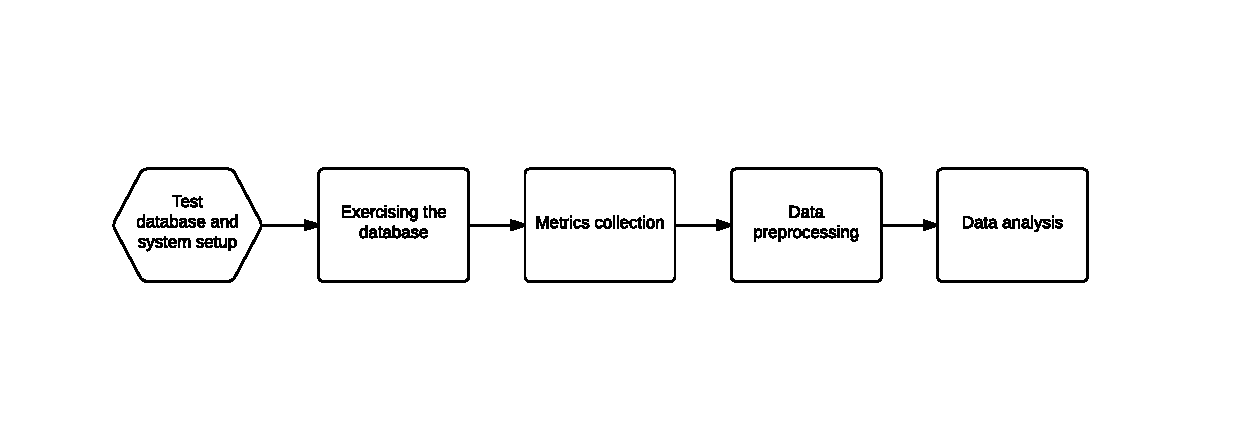
\includegraphics[width=1\textwidth]{approach.pdf}
%	\centering
%	\caption{Approach overview}
%    \label{fig:approach}
%\end{figure} 
%%\includepdf][pages={1}][width=\columnwidth{approach.pdf}

\begin{figure*}[thb]
	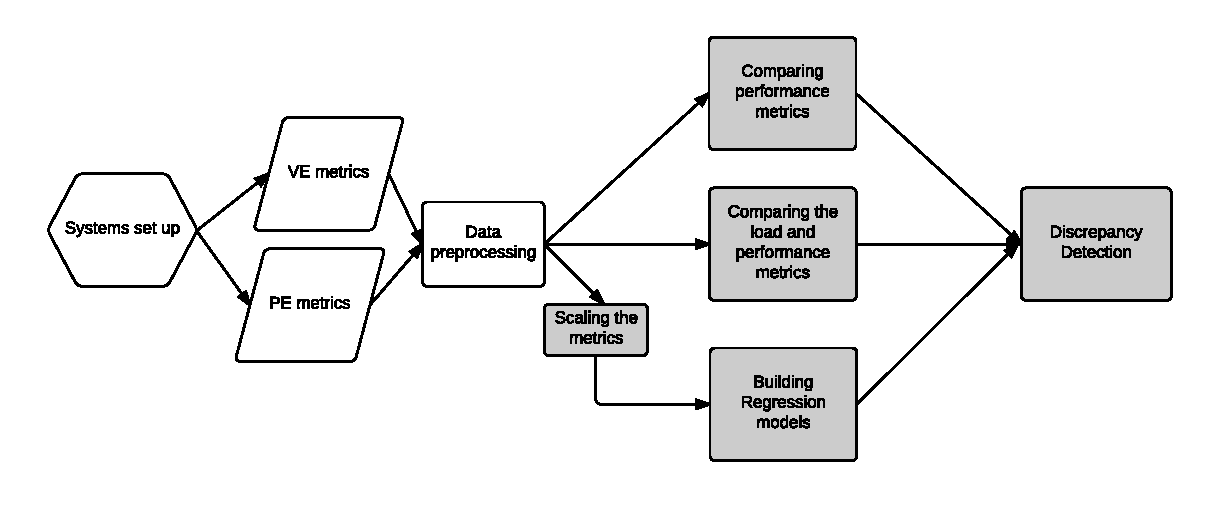
\includegraphics[width=\textwidth]{figures/approach_perf_vr1}
	\caption{Approach Overview}
	%\captionsetup{justification=centering}
	\label{fig:Approach}
\end{figure*}

In this section, we present our case study setup. \ian{todo}%The primary intention behind our experiment was to observe the performance of the system in a virtual environment. Additionally, to analyze whether the metric values depict a similar behavior when compared cross-environment. Once the performance metrics are recorded and processed, we then analyze our results using graphical techniques and regression models. Figure 1 shows the synopsis of our approach.


\subsection{Subject Systems}
Dell DVD Store (DS2)~\cite{delldvd} is an online multi-tier e-commerce web application that are widely used in performance testing and prior performance engineering research~\cite{Shang:2015:ADP:2668930.2688052,Nguyen:2012:ADP:2188286.2188344, jackicsm2009}. We deploy DS2 on a Apache (Version 3.0.0) web application server with MySQL 5.6 database server~\cite{mysql}. CloudStore~\cite{cloudstore}, our second subject system is an open source application based on TPC-W benchmark~\cite{tpcw}. CloudStore are widely used to evaluate the performance of cloud computing infrastructure when hosting web-based software systems and is leverage used in prior research~\cite{tarekmsr16, andmore}. We deploy CloudStore on \textit{Apache Tomcat}~\cite{tomcat} (version 7.0.65) with MySQL 5.6 database server~\cite{mysql}. 


\subsection{Environmental Setup}

The performance tests of the two subject systems are conducted on three machines in a lab environment. Each machine has an Intel i5 4690 Haswell Quad-Core 3.50 GHz CPU, with 8 GB of memory, connected to a local gigabyte ethernet. The first machine hosts the web server and application server (Apache and Tomcat). The second machine hosts the MySQL 5.6 database server. The load drivers (e.g., JMeter) was deployed on the third machine. The operating systems on the three machines are Windows 7. We disable all other processes and un-related system services to minimize their performance impact.

%was dedicated to the database server, the second machine was dedicated to the web server and the third machine was used to run the load driver.
\noindent \textbf{Virtual environment.} We install one Virtual Box \ian{version?} and create only one virtual machine on one physical machine to avoid the interference between virtual machines. For each virtual machine, we allocate two cores and 3GB of memory. 

%Our virtual setup was identical to our physical setup. The virtual environment was run on the same physical machines with all the resources provided to the host and the same set of aforementioned configuration for the virtual environment. We opted for single tenancy of the guest operating system to avoid any unwanted noise. 

\noindent \textbf{Physical environment.} To make the physical environment similar to the virtual environment, we only enable two cores and 3GB memory for each machine for the physical environment. 

%To make the systems' configuration identical prior to exercising the subject systems, we chose 2 cores and 3GB of memory dedicated to each environment to avoid crashes on the guest operating system in the virtual environment. We also made sure to kill all the processes before we start our performance testing to minimize any discrepancy present.

%\subsection{Exercising the database}
%Following the set up of our subject systems on the respective servers, the systems were exercised with an aid of drivers. These drivers generated multi-type web requests and simulated real-time user behavior depending on the input parameters provided. We ran our performance tests for numerous hours while recording all the performance metrics generated for varying load applied on our software systems.
\subsection{Performance tests}

DS2 is released with a dedicated load driver program that is designed to exercise DS2 for performance testing. We leverage the load driver to conduct performance testing on DS2. We leverage Apache Jmeter~\cite{apachejmeter} to generate a workload for conducting performance tests on CloudStore. For both subject system, the workload of the performance tests are variated periodically in order to avoid the bias from a consistent workload. The workload variation was introduced by the number of threads. A higher number of threads represented a higher number of users accessing the system. Each performance test is run after a 15 minutes warning up period of the system and last for 9 hours. 


%and the last 30 minutes in order to 

 %The choice of load was random but consistent between both of the environments. As our study was based on exercising our systems and recording the performance metrics, and not stress testing \cite{stresstesting}, the respected limits were chosen in order to avoid the under-performance of the physical machine and system failure of the virtual machine.


%\subsection{Metrics Collection}
\subsection{Data collection and preprocessing}

\noindent \textbf{Performance metrics.} We used \textit{PerfMon}~\cite{perfmon} to record the values of performance metrics. \textit{PerfMon} is a performance monitoring tool used to observe and record performance metrics such as CPU utilization, Memory usage and disk IOs. We record all the available performance metrics that can be monitored on a single process by \emph{PerfMon}.  We recorded record the performance metrics of both the process of web server/application server and the database server with an interval of 10 seconds. In total, we recored 56 performance metrics. 

\noindent \textbf{System throughput.} We used web server access logs from Apache and Tomcat to calculate the throughput of the system by measuring the number of requests per minute. The two data sets were then concatenated and mapped against requests according to the timestamps.

In order to combine the two datasets of performance metrics and system throughput, and to minimize noise of performance metrics recording, we calculate the mean values of the performance metrics in every minute and combine the datasets of performance metrics and system throughput based on the time stamp at minute level. Similar approach has been leverage to address mining performance metrics challenges~\cite{foo2010mining}.


\section{Case Study Results}
\label{sec:results}

\begin{comment}
	The objective of our case study is a comparative analysis of the two environments and to find out if there exists software performance regression between a dedicated server and the virtual environment. To analyze this, we divided our project into three research questions. Following the set up of the subject systems and data preprocessing, we used requests per minute as our independent variable and performance metrics as our dependent variables to answer our research questions. %Firstly, we observe if our models are transferable across the three chosen environments. Secondly, if the models can accurately predict counter values cross-servers. Lastly, if defect injection will generate similar performance metrics values compared   

\subsection{\textbf{Data Analysis}}
Following the data transformation, we used R \cite{R} to derive conclusions for our research questions with the help of Spearman correlation, Q-Q plots \cite{qqplots}; a graphical technique to detect if two sets of data belong to the same population, Mann-Whitney \textit{U} test \cite{mannwhitney}, and generalized linear regression models (GLM) \cite{SanFranciscoStateUniversity}. Spearman correlation is used to identify the level of association between two variables while Mann-Whitney \textit{U} test is used to verify the hypothesis that if the data sets belong to the same population.
%calculate the absolute deviation in a dataset from the median \cite{brownftest} \textcolor{red}{or instead brown forsythe test. enough already for rq1, discuss}. 
Both the aforementioned methods do not strictly assume that the ordinal data is normally distributed \cite{spearman} \cite{manutest}. Due to the size of our data, heat maps \cite{heatmaps} were used to visualize the correlations. We chose model-based analysis as they can support the automatic selection and detection of performance abnormalities between heterogeneous environments. \cite{Shang:2015:ADP:2668930.2688052}\cite{Nguyen:2012:ADP:2188286.2188344}. Contrary to the usual practice of ad-hoc selection of certain target performance metrics \cite{heger2013automated} to detect performance regression, we included the compete set of all 56 metrics to build our models. For our linear regression models, we processed our data in two steps. First, we remove any metrics that showed no variance by a R script, for example a metric which has less than 20 unique values \cite{rahm2000data}. Next, we also remove the metrics which have high correlation amongst themselves to remove any \textit{multicollinearity} present \cite{mansfield1982detecting} so that the models do not over fit based on similar predictors(performance metrics) for the load. This approach will also magnify the metric which actually contribute the most to the model. The rationale behind aforementioned steps was to clean up data that may not contribute significantly to the model \cite{Shihab:2010:UIC:1852786.1852792}. 


Once our data was organized our next step was to build the GLM using the physical and the virtual environment's performance metrics. Our models were built using the load as the dependent variable and the performance metrics as the independent variable i.e. the load is dependent on the change of values of the performance metrics. with the help. We, additionally, trained and tested our models for the same environment before using it cross-environments. This served as the benchmark for lower limit of the prediction percentage error. A model tested for the same environment was validated via ten-fold cross validation \cite{Cross_Validation} \cite{kohavi1995study}. Each fold is based on a random subset of values. The model is trained on 9 folds and tested on the $10^{th}$ fold. This is done 10 times with 10 different subsets of data each time. The accuracy of our models was determined by the percentage error of the predicted load versus the actual load values which was calculated as the absolute difference of the actual and predicted load values with respect to the actual load values.

Based on the results from the GLMs we then investigate about the metrics that are contributing the most and their respective correlation values using heat maps. Heat maps allow us to graphically view, in our case, the individual metrics and their correlation values. 

\end{comment}

The goal of our study is to evaluate the discrepancy between performance testing results in virtual and physical environments. Shown in Section~\ref{sec:related_work}, prior research examine performance testing results in three types of approaches: 1) examining individual performance metric, 2) examining relationship among performance metrics and 3) building statistical models using performance metrics. \emad{I think we need better arguments for why we focus on these 3 things. Just saying prior work did this so we do it is kind of weak motivation I feel.} In the rest of this section, we compare the performance testing results based on such three approaches.



\subsection{Examining individual performance metric}
\label{sec:individual}
\emad{Do we want to list a motivation here? Also, do we want to use subsections or RQs to organize the sections.}
\noindent \textbf{Approach.} 

First, we compare every individual performance metric between virtual and physical environments. Since the performance tests are conducted in different environments, intuitively the values of performance metrics are not the same. For example, the virtual environment may have higher CPU usage than the physical environment. Therefore, instead of comparing the values of each performance metric in both environments, we study whether the performance metric follow the same trend in virtual and physical environments. 

First, we plot a quantile-quantile plot (Q-Q plot)~\cite{qqplots} for every performance metric in two environments. A Q-Q plot is a plot of the quantiles of the first data set against the quantiles of the second data set. We also plot a 45-degree reference line on the Q-Q plots. If the performance metrics in both environments follow the same distribution, the points on the Q-Q plots should fall approximately along this reference (i.e., 45-degree line) line. A large departure from the reference line indicates that the performance metrics in the virtual and physical environments come from populations with different distributions. 

Second, to quantitatively measure the discrepancy, we perform a Kolmogorov-Smirnov test~\cite{kstest} between every performance metric in the virtual and physical environments. Since the scales of each performance metric in both environment are not the same, we first scale the metrics based on their median values and their mean absolute deviation: 
\begin{equation}
	\label{equ:mad}
		M_{scale}=\frac{M-\tilde{M}}{MAD(M))}		
\end{equation}
	
where $M_{scale}$ is the scaled value of the metric, $M$ is the original value of the metric, $\tilde{M}$ is the median value of the metric and $MAD(M)$ is the median absolute deviation of the metric~\cite{walker1929studies}. The Kolmogorov-Smirnov test gives a p-value as the test outcome. A p-value ≤ 0.05 means that the result is statistically significant, and we may reject the null hypothesis (i.e., two populations are from the same distribution). By rejecting the null hypothesis, we can accept the alternative hypothesis, which tells us the performance metrics in virtual and physical environments do not have the same distribution. We choose Kolmogorov-Smirnov test since it does not have any assumption on the distribution of the metrics.

Finally, we calculate Spearman's rank correlation between every performance metric in virtual environment and and the corresponding performance metric in physical environment, in order to assess whether the same the performance metric in two environments follow the same trend during the test. Intuitively, two sets of performance testing results without discrepancy should show similar trend, i.e., when Memory keeps increasing in the physical environment, the memory should also increases in the virtual environment. We choose Spearman's rank correlation since it does not have any assumption on the distribution of the metrics. 

\noindent \textbf{Results.}

\textbf{Most performance metrics do not follow the same distribution in virtual and physical environments.} Figure~\ref{fig:qqds2} and \ref{fig:qqcs} show the Q-Q plots by comparing the quantiles of performance metrics from virtual and physical environments. Due to the limited space, we only present Q-Q plot for CPU User time, IO data operations/sec and memory working set for both web sever and database server. The results show that the lines on the Q-Q plot are not close to the 45-degree reference line. By looking closely on the Q-Q plots we find that the patterns of each performance metric from different subject systems are different. For example, the web cpu user time for DS2 in virtual environment shows higher values than in the physical environment in the median to high range of the distribution; while the Q-Q plot of CloudStore shows web cpu user time with higher values in the low range of the distribution. In addition, the lines of the Q-Q plots for database memory working set show completely different shape in DS2 and CloudStore. The results imply that the discrepancies between virtual and physical environments are different across subject systems. The impact of the subject systems will be discussed in future work.

The majority of the performance metrics have statistically significantly different distribution (p-values lower than 0.05 in Kolmogorov-Smirnov tests)。 Only 13 and 12 metrics have p-values higher than 0.05, for DS2 and CloudStore, respectively, showing statistically in-signifiant difference between the distribution in virtual and physical environments. By looking closely at such metrics, we find that these metrics either do not highly relate to the execution of the subject system (e.g., web server CPU privileged time in DS2), or highly related to the workload. Since the workload between the two environments are similar, it is expected that the metrics relate to the workload follow the same distribution. For example, the I/O operations are highly related with the workload. The metrics related to I/O operations may show statistically in-signifiant difference between the distribution in virtual and physical environments (e.g., web server I/O write operations per second in DS2). %\emad{should we list the metrics}

 %We find that out of 44 metrics, only 3 and 2 metrics have values with low variance during the performance tests, for DS2 and CloudStore, respectively. We cannot perform Kolmogorov-Smirnov tests on such metrics \emad{why not}

\begin{comment}
\begin{table}[tbh]
	\centering
	\caption{Results of our KS-Test}
	\label{ks-test}
	\resizebox{\columnwidth}{!}{%
		\begin{tabular}{|c||c|c}
			\hline
			\textbf{KS-Test} & \textbf{p-val\textless0.05} & \textbf{p-val\textgreater0.05} \\ %\hline
			\midrule
			\midrule
			\textbf{DS2} & 26 & 16 \\ \hline
			\textbf{CloudStore} & 31 & 12 \\ \hline
		\end{tabular}%
	}
\end{table}
\end{comment}

%the p-values are larger than 0.05 in only X metrics. In 

 %However, even if the distributions are different, the difference can be negligible. To find out the quantitative difference between the two non-identical distributions  we used Cliff's Delta \cite{cliffsdeltajack}. We did not apply this technique on counters such as \textit{elapsed time, handle count, creating process ID, ID process, thread count} and \textit{priority base} as the do not contribute to the conclusions of the performance tests. We labeled them as NA(not applicable) in our table. The results showed that most of the performance metrics did not belong to the same distribution and have a significant difference.



%As seen in Figure 2 for the subject system DS2, the CPU user times for the web servers are closer to the line Z however the plots database servers' CPU user times are highly deviated from the same line as it not visible in the same plot. The disk IO operations/sec for the web servers gradually deviate form the line Z whereas the database server is, again, highly deviated. The same can be concluded about the memory working sets for both of our environments.
%Figure 3 shows the Q-Q plots for CloudStore. The web servers CPU user times are not congruent with the line Z. The database server CPU user times towards the tail of the plot are closer to the line Z however they still do not follow the line Z. The disk IO operations for both servers tends to follow the line Z initally but gradually moves away. Further on, the memory working set for both of our servers, as seen, are distant to the line Z.

\textbf{Most performance metrics do not have the same trend in virtual and physical environments.} Table~\ref{tab:correlationrq1} shows the Spearman correlation coefficient and corresponding p-value between the selected performance metrics as Q-Q plots. We find that the for the web server memory working set in CloudStore and the database server memory working set in D2S, there exist strong (0.69) to moderate (0.46) correlation between virtual and physical environments, respectively. By examining the metrics, we find that both metrics have a increasing trend that may be cause by memory leak. Such increasing trend may be the cause of the moderate to strong correlation. Instead of showing the selected metrics as the Q-Q plots, Table~\ref{tab:correlationall} shows a summary of the spearman's ranking correlation of all the performance metrics. Most of the correlations have an absolute value of 0 to 0.3 (low correlation), or the correlation is not statistically significant (p-val\textgreater0.05).

\hypobox{Performance metrics typically do not follow the same distribution or follow the same trend in virtual and physical environments. System load metric (throughput) and some performance metrics that are correlated with system load may be exceptions.}

%If the correlation value is closer to 1 the metrics have a strong correlation and if the value is closer to 0 the metrics have a weak correlation. A negative correlation means that if one of the metrics is increasing in value, the other is decreasing. For both of our subject systems we observe that the correlation values are mostly positive and are closer to 0 representing weak correlations. This conclusion, however, is not applicable to the user times from both environments as the p-value $>$ 0.05.


%\textbf{Motivation}: Performance assurance activities are not only bounded by the idea that performance regression can only be identified relative to different versions of the software. A software system might also regress once it is transferred from one environment to another. According to the norm, practitioners often rely on performance metrics generated by the virtual environment prior to releasing it on a disparate environment. We address this question by comparing the metric values between the physical and virtual server. 

%\textbf{Approach}: As mentioned earlier in Section 3, after setting up the subject systems, we used the number of requests as our workload for the systems. A script was written to randomly alter the workload after every minute for CloudStore and every two minutes for DS2. The script was based on an underlying assumption that every unit of change in the performance metrics there will be a consequent unit of change in the workload which eventually introduced variety in our dataset. \cite{linearregression}. Subsequently, the requests per minute were mapped against the performance metrics recorded via \textit{perfmon}.

%The numerical values for requests per minute were extracted out of the web server's access logs. These requests were recorded per second and reached up to thousands in a minute, depending on the workload. We then, with the aid of a script, grouped and extracted the requests per minute for as long as the test systems were exercised. The metrics, on the contrary, were recorded every 10 seconds. A set of six records was averaged out as a minute according to the timestamps. This was called a single \textit{run}. The metrics generated for the web and database server were concatenated. Ultimately, we had a dataset consisting of 500 runs where every record represented a \textit{run}; the metrics and requests generated for a given minute. This process was carried out for both of our environments. The two datasets, to analyze any discrepancies, were then analyzed using R's Q-Q plots and \textit{cor} function.

\begin{figure}[thb]
	\centering
	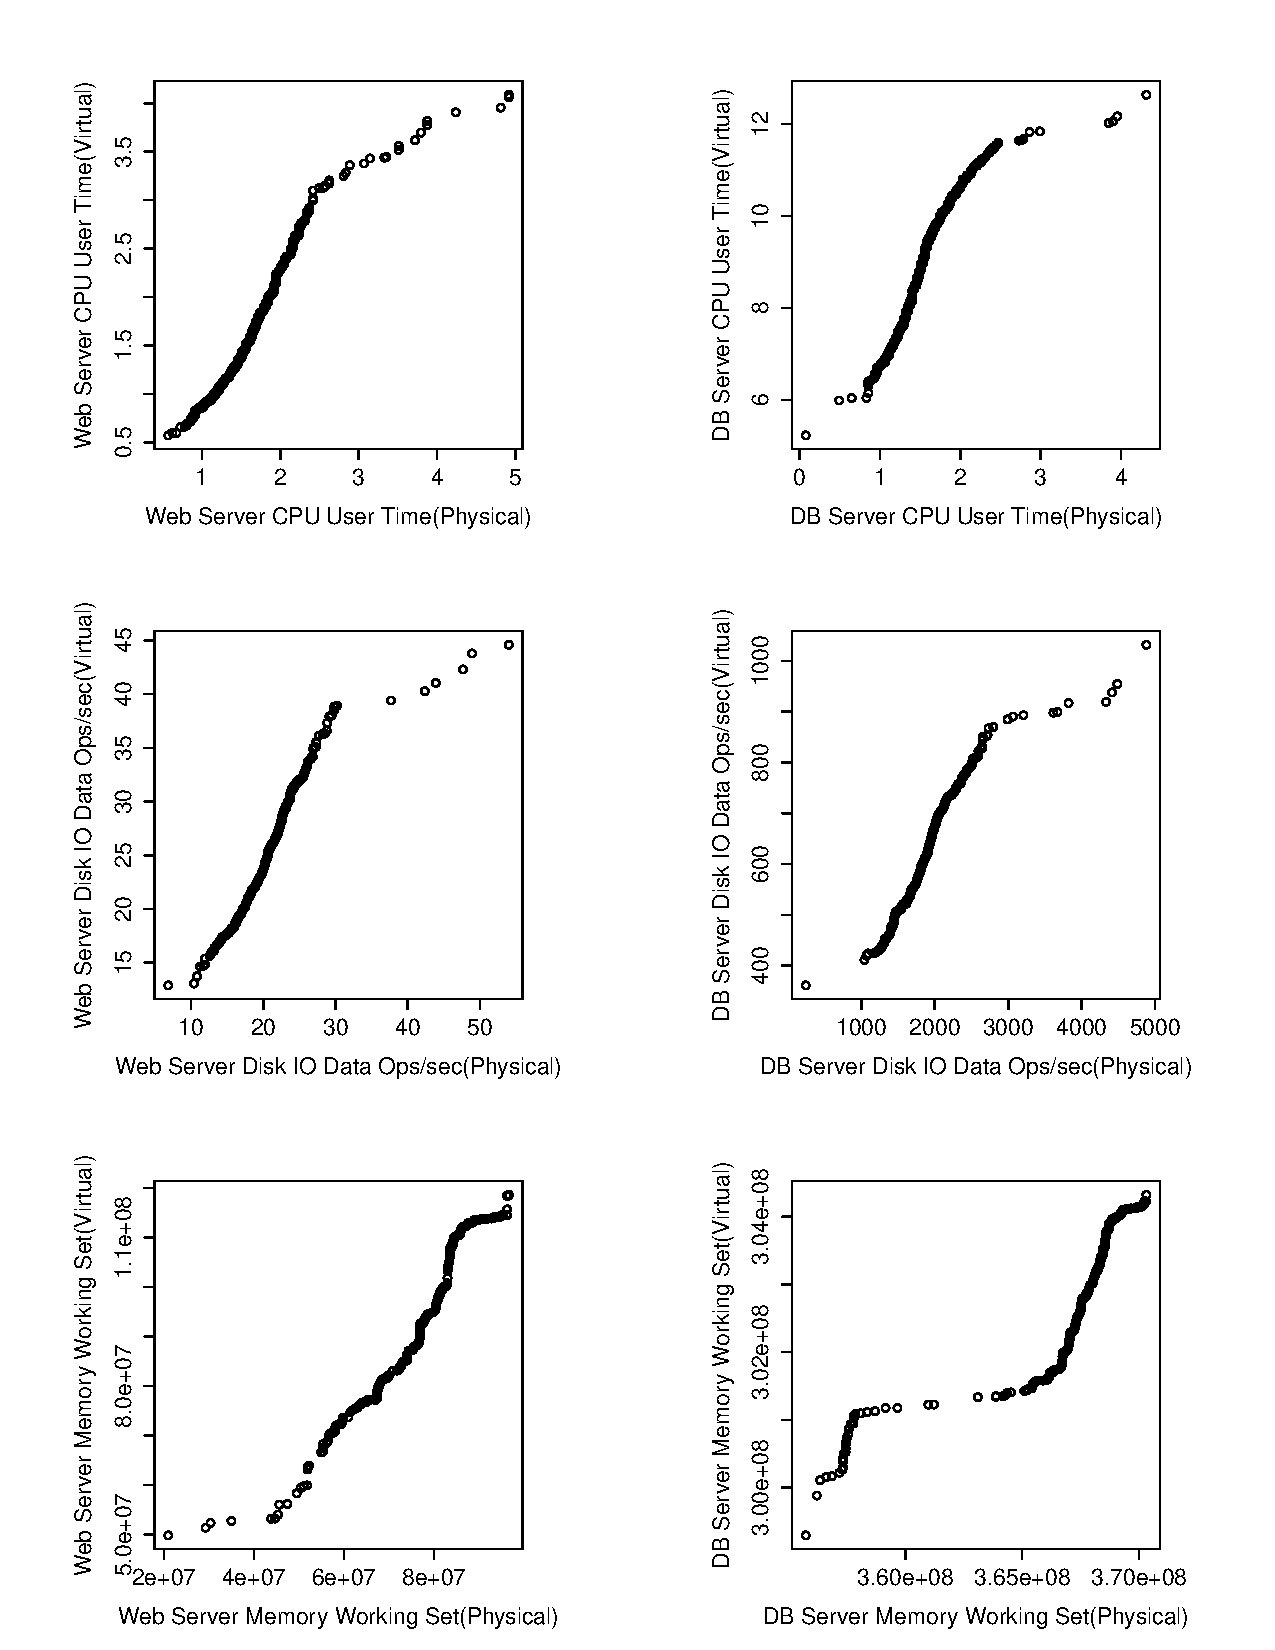
\includegraphics[width=0.9\columnwidth]{figures/qqplots_DS2.pdf}
	\caption{Q-Q plots for DS2.}
%	\captionsetup{justification=centering}
	\label{fig:qqds2}
\end{figure}



\begin{figure}[thb]
	\centering
	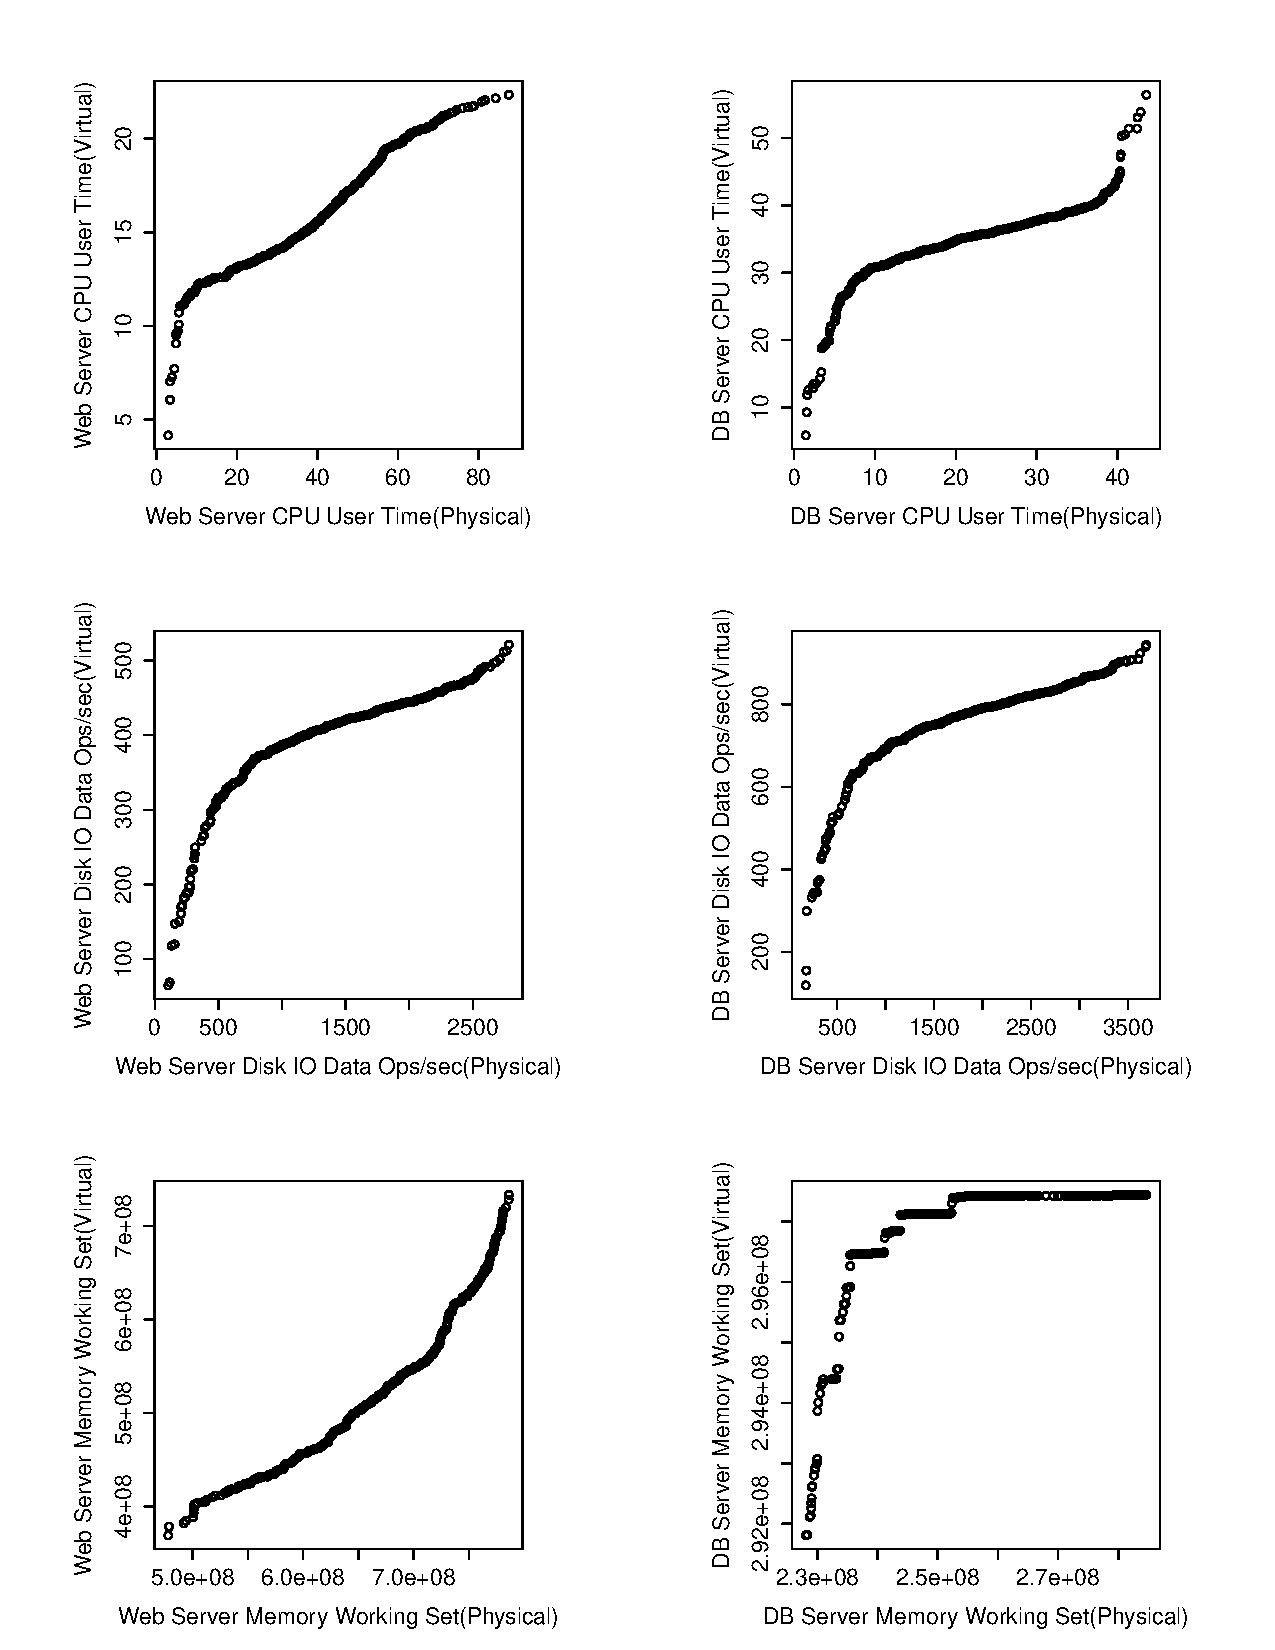
\includegraphics[width=0.9\columnwidth]{figures/qqplots_CS.pdf}
	\caption{Q-Q plots for CloudStore.}
%	\captionsetup{justification=centering}
	\label{fig:qqcs}
\end{figure}

\begin{comment}
\begin{table}[tbh]
	\centering
	\caption{Results of Ks test and Cliff Delta on Performance Metrics}
	\label{my-label}
	\resizebox{\columnwidth}{!}{%
		\begin{tabular}{|c||c|c|c|c|c|}
			\hline 
			\multirow{2}{*}{\textbf{System}} & \multirow{2}{*}{\textbf{p\textgreater0.05}} & \multicolumn{4}{c|}{\textbf{p\textless0.05}} \\ \cline{3-6} 
			&  & \textbf{Neglible} & \textbf{Small} & \textbf{Medium} & \textbf{Large} \\ %\hline
			\midrule 
			\midrule 
			DS2 & 2 & 1 & 2 & 5 & 34 \\ \hline
			CloudStore & 0 & 1 & 2 & 1 & 40 \\ \hline
		\end{tabular}%
	}
\end{table}
\end{comment}

% Please add the following required packages to your document preamble:
% \usepackage{multirow}
% \usepackage{graphicx}
\begin{table}[thb]
	\centering
	\caption{Spearman's ranking correlation coefficients and p-values of the highlighted performance metrics.}
	\label{tab:correlationrq1}
	\resizebox{\columnwidth}{!}{%
		\begin{tabular}{|c||c|c|c|c|}
			\hline
			\multirow{2}{*}{\textbf{Performance Metrics}} & \multicolumn{2}{c|}{\textbf{DS2}} & \multicolumn{2}{c|}{\textbf{CloudStore}} \\ \cline{2-5} 
			& \textbf{coef.} & \textbf{p-value} & \textbf{coef.} & \textbf{p-value} \\ %\hline
			\midrule 
			\midrule 
			Web Servers' User Times & 0.08 & 0.07 & -0.04 & 0.33 \\ \hline
			DB Servers User Times & -0.05 & 0.30 & 0.10 & 0.02 \\ \hline
			Web Servers' IO Data Ops/sec & 0.25 & 0.00 & 0.13 & 0.00 \\ \hline
			DB Servers' IO Data Ops/sec & -0.14 & 0.00 & 0.13 & 0.00 \\ \hline
			Web Servers' Memory Working Set & 0.22 & 0.00 & 0.69 & 0.00 \\ \hline
			DB Servers' Memory Working Set & 0.46 & 0.00 & -0.16 & 0.00 \\ \hline
		\end{tabular}%
	}
\end{table}

\begin{table}[tbh]
	\centering
	\caption{Summary of spearman's ranking correlation p-values and absolute coefficients of all the performance metrics in DS2 and CloudStore. The numbers in the table are the number of metrics that fall into each category.}
	\label{tab:correlationall}
	\resizebox{\columnwidth}{!}{%
	\begin{threeparttable}
  
		\begin{tabular}{|c||c|c|c|c|c|}
			\hline
			\multirow{3}{*}{\textbf{System}} & \multirow{3}{*}{\textbf{p-value\textgreater0.05}} & \multicolumn{4}{c|}{\textbf{p-value\textless0.05}} \\ \cline{3-6} 
			&  & \textbf{0.0$\sim$0.3} & \textbf{0.3$\sim$0.5} & \textbf{0.5$\sim$0.7} & \textbf{0.7$\sim$1} \\ %\hline
			\midrule 
			\midrule 
			\textbf{DS2} & 8 & 28 & 4 & 0 & 1\emad{adds to 41 not 44} \\ \hline
			\textbf{CloudStore} & 5 & 29 & 4 & 4 & 2 \\ \hline
		\end{tabular}%
		\begin{tablenotes}
			\item One metric in DS2 (Web I/O read operations/sec) is constant. Therefore, we do no calculate the correlation on that metric.
		\end{tablenotes}
		\end{threeparttable}
	  
	}
\end{table}

%\begin{table}[t]
%	\centering
%	\caption{DS2: Correlation Values}
%	\label{resultRQ3}
%	\begin{tabular}{c|cc}
%		\toprule
%		\textbf{Performance Metrics}   & \textbf{Cor} & \textbf{p-value}\\  
%		\midrule 
%		\midrule 
%		\textbf{Web Servers' User Times} & \ 0.08 & 0.07\\
%		\textbf{DB Servers' User Times} & -0.05 & 0.30\\
%		\midrule 
%		\textbf{Web Servers' IO Data Ops/Sec}   &\ 0.25 & 0.000 \\
%		\textbf{DB Servers' IO Data Ops/Sec} & -0.14 & 0.00\\
%		\midrule 
%		\textbf{Web Servers' Memory Working Set} &\ 0.22 & 0.00\\
%		\textbf{DB Servers' Memory Working Set} &\ 0.46 & 0.00\\
%		\bottomrule             
%	\end{tabular}
%\end{table}
%	
%\begin{table}[t]
%		\centering
%		\caption{CloudStore: Correlation Values}
%		\label{resultRQ3}
%		\begin{tabular}{c|cc}
%			\toprule
%			\textbf{Performance Metrics}   & \textbf{Cor}& \textbf{p-value}\\
%			\midrule 
%			\midrule 
%			\textbf{Web Servers' User Times} & \ 0.01& 0.87\\
%			\textbf{DB Servers' User Times} & \ 0.20 & 0.00\\
%			\midrule 
%			\textbf{Web Servers' IO Data Ops/Sec}   & \ 0.17& 0.00 \\
%			\textbf{DB Servers' IO Data Ops/Sec} & \ 0.18& 0.00\\
%			\midrule 
%			\textbf{Web Servers' Memory Working Set} &\ 0.69& 0.00\\
%			\textbf{DB Servers' Memory Working Set} & -0.13 & 0.00\\
%			\bottomrule             
%		\end{tabular}
%\end{table}

%\begin{figure}[t!]
%	\centering
%	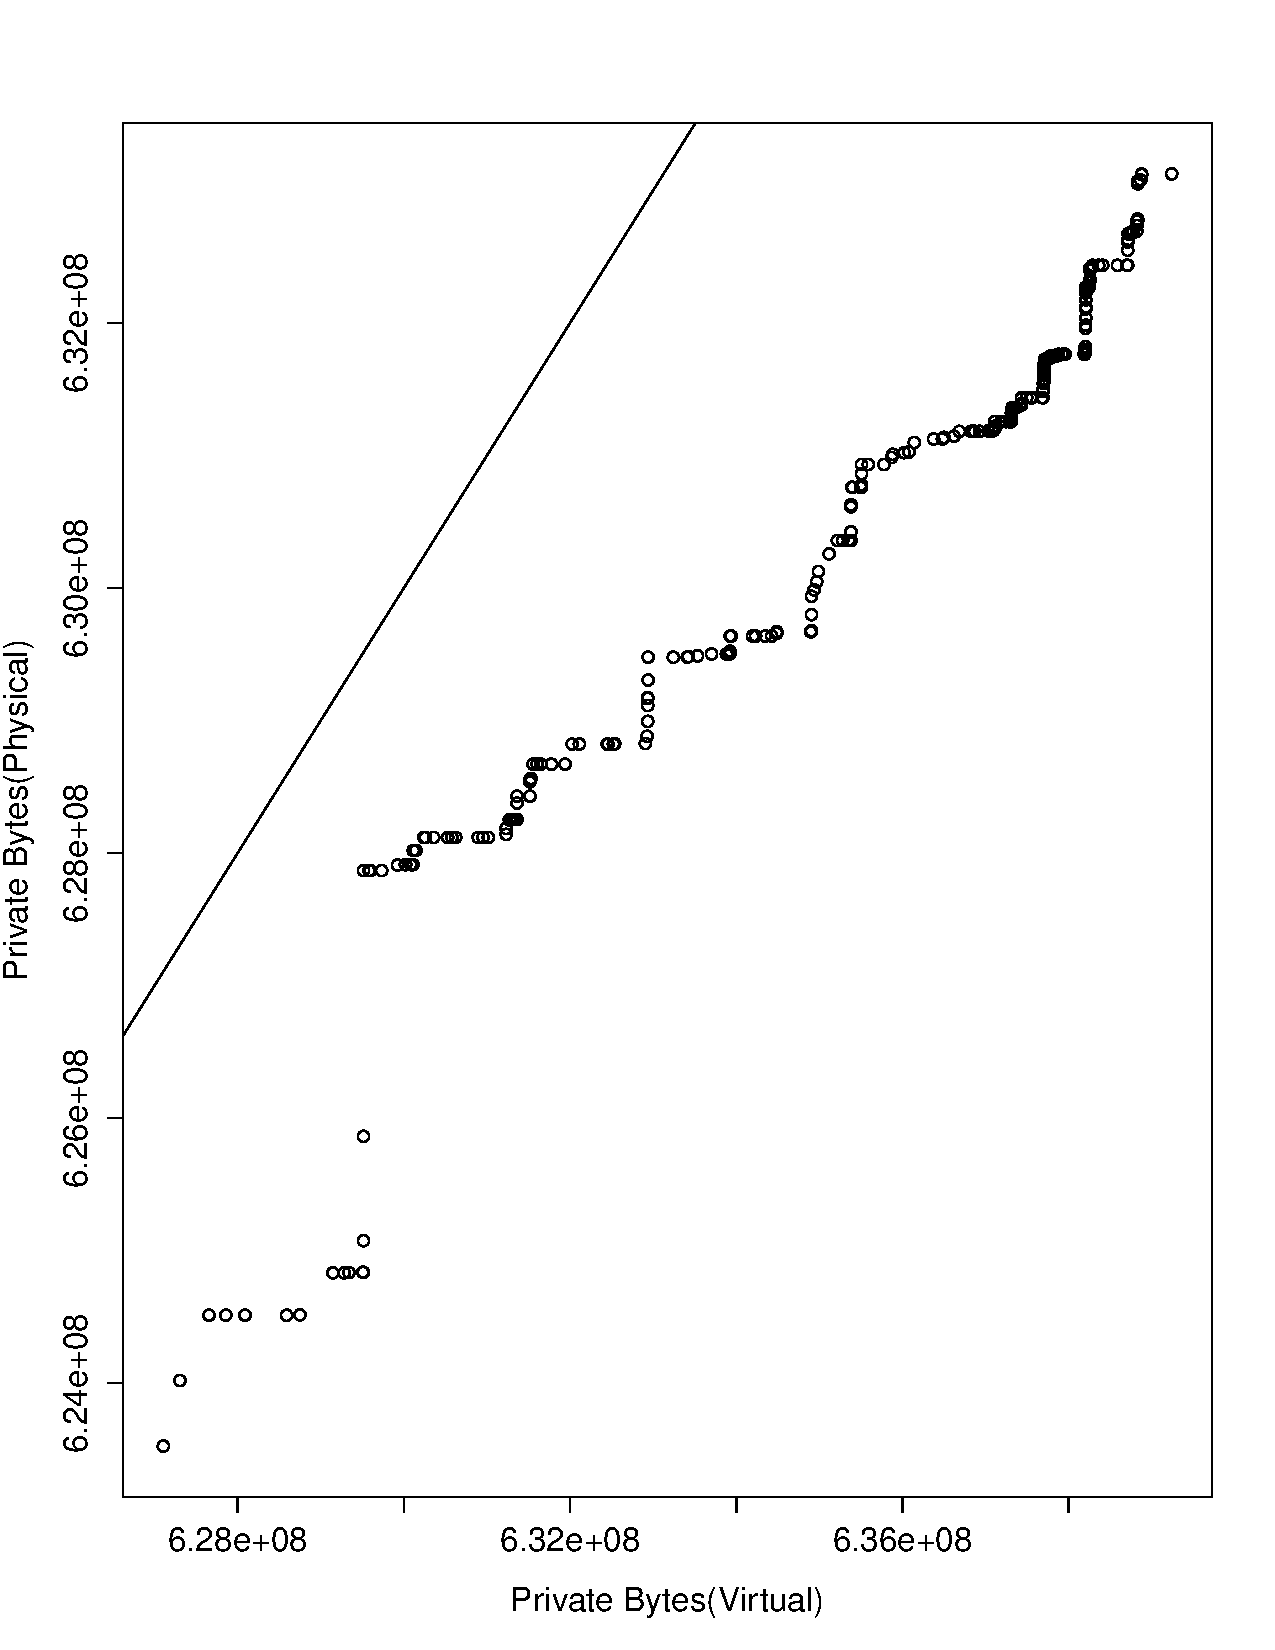
\includegraphics[width=0.7\textwidth]{private_bytes.pdf}
%	\caption{QQ-plot of Private Bytes of Physical vs. Virtual Environment}
%	\captionsetup{justification=centering}
%	\label{fig:Results Table}
%\end{figure}

%\textbf{Approach}: 
%Following our data preprocessing, we decided to use Q-Q plot to identify if there exists a similarity between the distribution of our counters for the dedicated and the virtual server. We divided our metrics into three sub-categories namely \textit{processor, IO and memory}.


\subsection{Examining relationship among performance metrics}

%\textbf{Motivation}: Building on the conclusion from the previous research question, we next address the change in metric correlation values amongst themselves and versus the load. Our goal was to explore whether the change in correlation cross-environments is identical for both of our subject systems. This way we will be able to conclude whether a certain type of discrepancy is always present between the two environments or is it the unstable nature of the performance of subject systems in different environments. 

%Before the software is deployed in a physical environment, the performance analyst relies on the heuristics generated from the virtual environment \cite{foo2010mining}. One of the approaches to detect performance regression is to compare every metric with the previously passed performance test \cite{Shang:2015:ADP:2668930.2688052}. As discussed in our previous research question, most of the performance metrics between two environments do not belong to the similar distribution. 

%As discussed in RQ1, we discovered that our comparison of performance metrics between our physical and virtual environments produced dissimilar results. Our next step was to explore what metrics changed the most 


%As performance testing spans our from handful of hours to several days , the reliability on such exercise is remarkably critical. A recent bug fix or a modification may require a reiteration of performance tests \cite{foo2010mining}. On the contrary, This led us to our next question, that whether the performance assurance activities run on virtual environments can be duplicated.

\noindent \textbf{Approach.} 

We calculate Spearman's rank correlation coefficient among all the metrics from each performance test in one environment to study the relationship among these metrics. Then we study whether such correlation coefficient is different between the virtual and physical environment. 

First, we compare the changes in correlation between the performance metrics and the system throughput. For example, in one environment, the system throughput may be highly correlated with CPU while in another environment, such correlation is low. In such a case, we would considering that there exist discrepancy in the correlation coefficient between CPU and the system throughput. Then, for every two metrics, we calculate the absolute difference between the correlation in two environments. For example, if CPU and Memory has a correlation of $0.3$ in the virtual environment and $0.5$ in the physical environment, we report the absolute difference in correlation as $0.2$ ($|0.3-0.5|$). Since we have 44 metrics in total, we plot a heatmap in order to visualize the 1,936 absolute difference values between every pair of performance metrics. The lighter the color for each block in the heatmap, the larger the absolute difference in correlation a pair of performance metrics have. With the heatmp, we can quickly spot the metrics that have large discrepancy in correlation coefficient. 


%In particular, we 


%We looked for the top 5 metrics which are highly correlated with the load in each of our environments. We used R's \textit{cor} function to determine the Spearman value of the aforementioned associations. 
%Next, we used heat maps to highlight the set of metrics which show a significant change in correlation values amongst themselves.
%The correlation values between the metrics of physical server were stored in matrix A. The correlation values between the metrics of the virtual server were store in matrix B. Matrix Z was the absolute difference between these two matrices. For example the Spearman correlation value for CloudStore's physical server between web server's User Time and database server's IO write/Bytes sec is 0.94. The correlation value for the same pair of metrics in the virtual environment is 0.26. Then the Matrix Z will record a value which is the absolute difference of the aforementioned Spearman values i.e. 0.68. If the metric value has changed significantly, according to the legend, this will be denoted as a 'hot zone' in the heatmap denoted by a lighter gradient of color.

\noindent \textbf{Results.}

\noindent \textbf{The correlation between system throughput and performance metrics changes between virtual and physical environments.} Table~\ref{tab:top10ds2p} presents the top ten metrics with the highest correlation to system throughput in the physical environment for DS2. We find that for these ten metrics, the difference in correlation coefficients in virtual and physical environments is up to 0.78 and rank changes from \#9 to \#40 .

\noindent \textbf{There exist differences in correlation among the performance metrics from virtual and physical environments.} Figure~\ref{fig:heatmap} present the heatmap showing the changes in correlation coefficient among the performance metrics from virtual and physical environments. By looking at the heatmap, we can find hotspots (with lighter color), which have larger correlation differences. Due to the limited space, we do not show all the metric names in Figure~\ref{fig:heatmap}. Instead, we enlarge the heatmap by showing one of the hotspots for each subject system in Figure~\ref{fig:heatmap}. We find that the hotspot in DS2 corresponds to the changes in correlation among I/O related metrics. Prior research on virtual machines has similar findings about I/O overheads in virtual machines~\cite{menon2005diagnosing,kraft2011io}.


%\ian{todo: this paragraph maybe useful} Figure 4 and 5 are the heatmaps for the change in correlation values amongst the metrics of two environments. For DS2, figure 4, the hot spots are mostly prevalent between the IO operations, for both the web and database server, cross-environments. This means the correlations amongst IO operations in the physical environment are not the same as the correlation between IO operations in the virtual environment. While CloudStore's heatmap, figure 5, shows that the change in correlation values is not as similar to DS2. Most of the hot spots are scattered across the heatmaps, contrary to DS2 where we can see clusters around most of the IO operations.  We also observed a similar change in correlation values between the processor times and other metrics. This trend may not be as strong as CloudStore's heatmap for DS2, however these changes in values can be found in both of our subject system.

%Table 3-6 are the top five highly correlated metrics with the load. In DS2, most of the IO operations from the web driver are highly correlated with the load in the physical environment. However, the database server is highly correlated than any of the metrics from the web driver in the virtual environment.
%Table 5 and 6 shows a much similar behavior of CloudStore in both the environments.

%We primarily learned that the DS2 IO operations' behavior in one environment are not similar to that of the physical environment. We also learned that the change in nature of correlation cross-environments is non-uniform.
%Figure 4 and 5 are the heatmaps for the change in correlations' values between the metrics of two environments. For DS2, figure 4, 4he hot spots are mostly prevalent between the IO operations cross-environment while CloudStore's heatmap, figure 5, shows that the change in correlation values is not as similar to DS2. Most of the hot spots are scattered across the heatmaps, contrary to DS2 where we can see clusters around most of the IO operations.
\hypobox{The correlations between performance metrics and system load may change considerably between virtual and physical environments. The correlation among performance metrics may also change considerably between virtual and physical environments. The correlations that are related with the I/O metrics have the largest discrepancy. }


\begin{figure*}[tbh]
	\centering
	{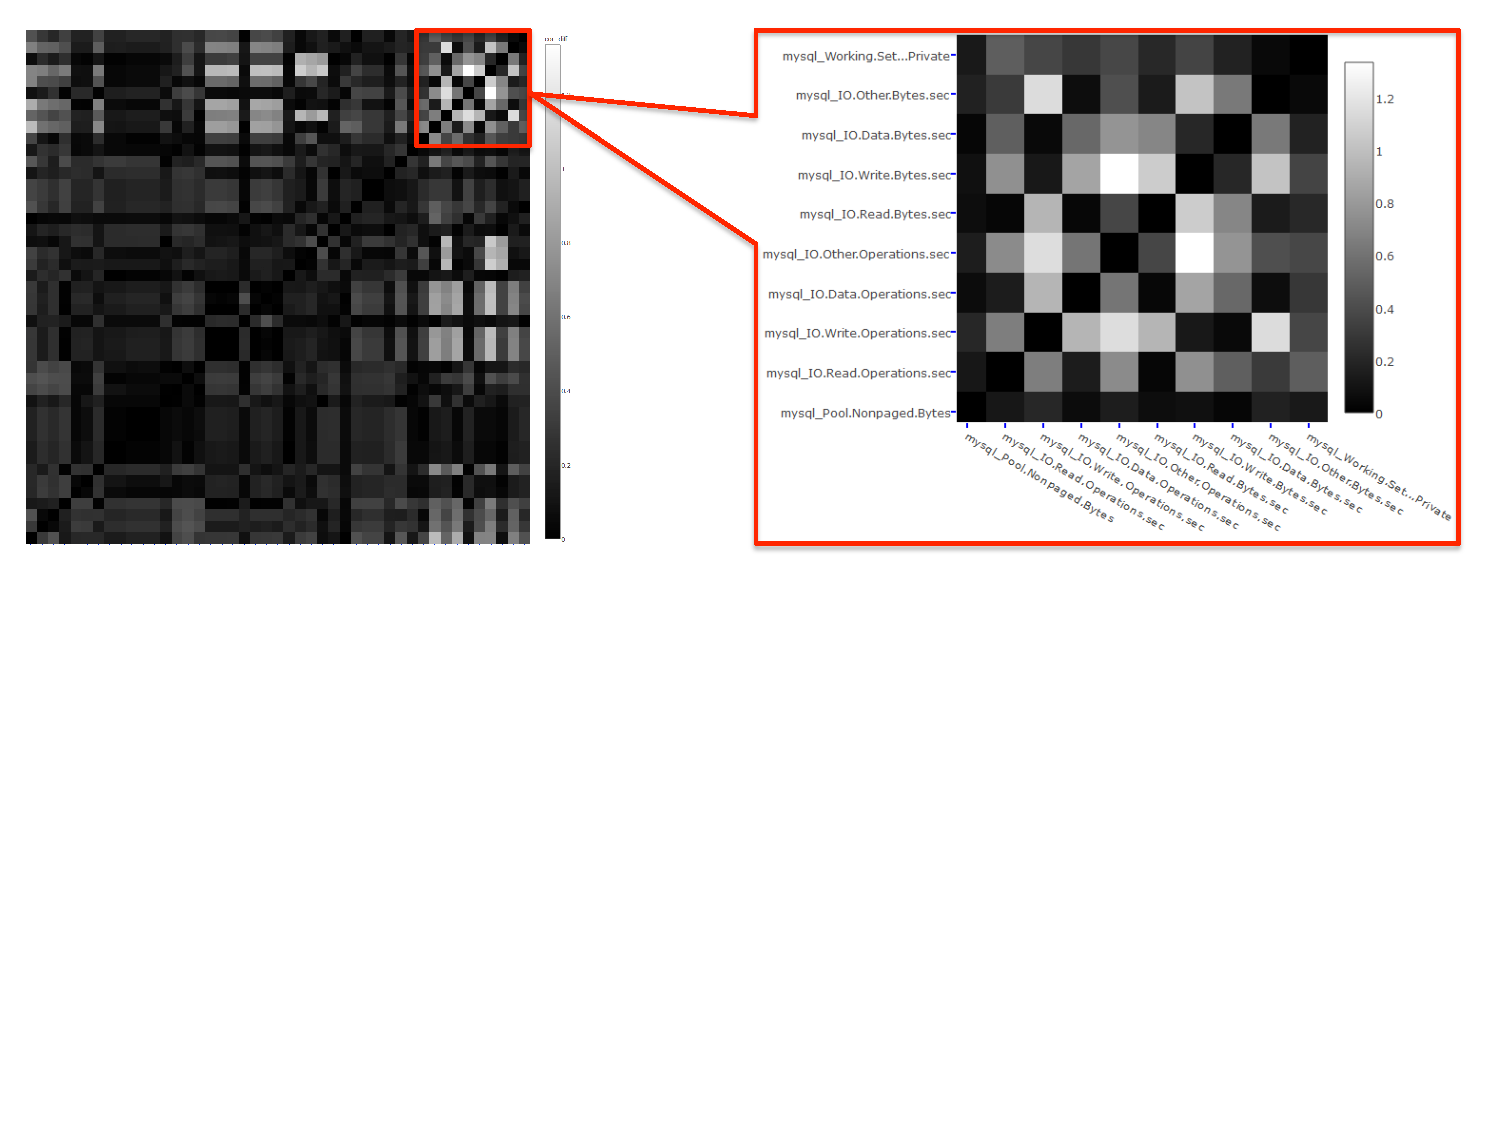
\includegraphics[width=.9\textwidth]{figures/heat}}
	\caption{Heatmap of correlation changes for DS2.}
	%\captionsetup{justification=centering}
	\label{fig:heatmap}
\end{figure*}


%\begin{figure}[tbh]
%	\centering	
%	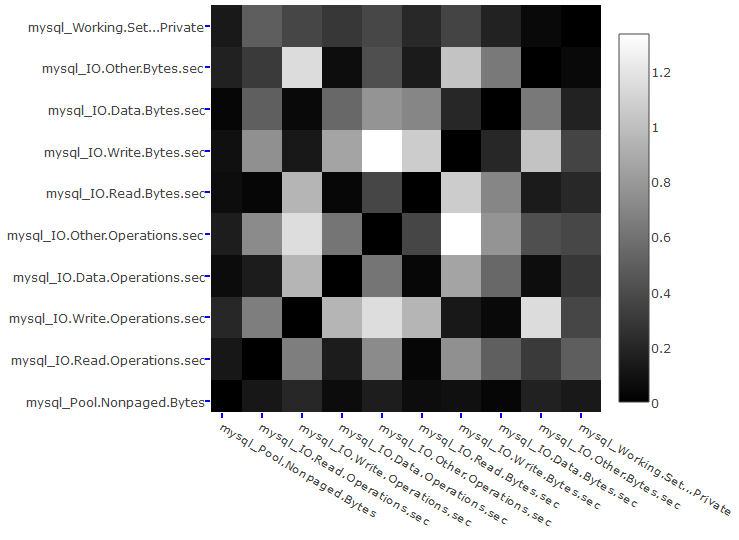
\includegraphics[width=\columnwidth]{figures/ds2_smaller_new.png}
%	\caption{Heatmap: DS2}
%	\captionsetup{justification=centering}
%	\label{fig:heathotds2}
%\end{figure}

%\begin{figure}[tbh]
%	\centering
%	{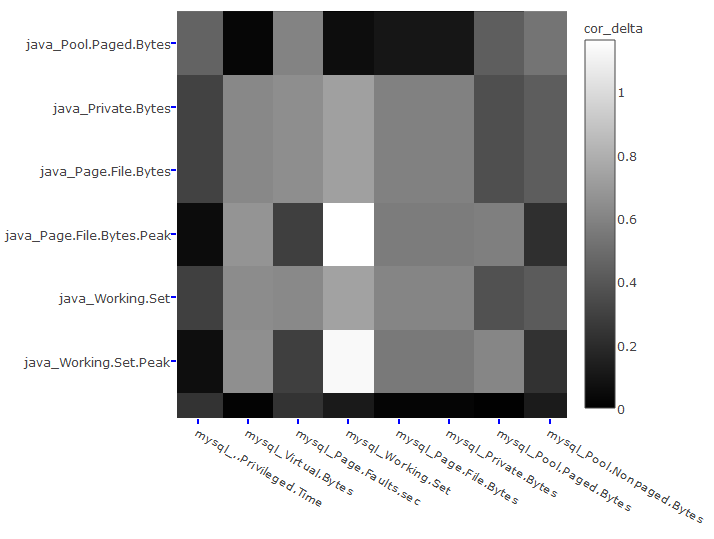
\includegraphics[width=\columnwidth]{figures/cloudstore_heatmap_smaller_new.png}}
%	\caption{Heatmap: CloudStore}
%	%\captionsetup{justification=centering}
%	\label{fig:heathotcs}
%\end{figure}


%\begin{table}[tbh]
%		\centering
%		\caption{DS2: Top 5 highly correlated metrics with load (Physical Server)}
%		\label{resultRQ3}
%		\begin{tabular}{c}
%			\toprule
%			1. Web Server IO Other Operations/sec \\
%			2. Web Server IO Other Bytes/sec \\
%			3. Web Server IO Write Operations/sec \\
%			4. Web Server IO Data Operations/sec \\
%			5. Web Server IO Data Bytes/sec \\
%			
%			\bottomrule             
%		\end{tabular}
%\end{table}


% Please add the following required packages to your document preamble:
% \usepackage{graphicx}
\begin{table}[tbh]
	\centering
	\caption{Top ten metrics with highest correlation coefficient to system throughput in the physical environment for DS2. }
	\label{tab:top10ds2p}
	\resizebox{\columnwidth}{!}{%
	\begin{threeparttable}
	
		\begin{tabular}{|c||c|c|c|c|}
			\hline
			\textbf{Rank} & \textbf{Performance } & \textbf{Coef. } & \textbf{Coef. } & \textbf{Rank in} \\ %\hline
			 & \textbf{ Metrics} & \textbf{PE} & \textbf{VE} & \textbf{VE} \\ %\hline
			\midrule
			1 & Web IO Other Ops/sec & 0.91 & 0.62 & 10 \\ \hline
			2 & Web IO Other Bytes/sec & 0.91 & 0.62 & 12 \\ \hline
			3 & Web IO Write Ops/sec & 0.91 & 0.63 & 9 \\ \hline
			4 & Web IO Data Ops/sec & 0.91 & 0.63 & 8 \\ \hline
			5 & Web IO Write Bytes/sec & 0.90 & 0.62 & 11 \\ \hline
			6 & Web IO Data Bytes/sec & 0.90 & 0.61 & 13 \\ \hline
			7 & DB IO Other Ops/sec & 0.84 & 0.75 & 3 \\ \hline
			8 & DB IO Data Ops/sec & 0.83 & 0.07 & 41 \\ \hline
			9 & DB IO Other Bytes/sec & 0.83 & 0.15 & 40 \\ \hline
			10 & DB IO Read Ops/sec & 0.82 & 0.15 & 39 \\ \hline
		\end{tabular}%
		\begin{tablenotes}
			\item PE in the table is short for physical environment; while VE is short for virtual environment.
		\end{tablenotes}
		\end{threeparttable}
		
	}
	
\end{table}


%\begin{table}[tbh]
%	\centering
%		\caption{DS2: Top 5 highly correlated metrics with load (Virtual Server)}
%		\label{resultRQ3}
%		\begin{tabular}{c}
%			\toprule
%			1. Database Server Handle Count \\
%			2. Database Server Working Set-Peak \\
%			3. Database Server Pool Paged Bytes \\
%			4. Database Server IO Other Operations/sec \\
%			5. Database Server Page File Bytes Peak \\
%			\bottomrule             
%		\end{tabular}
%\end{table}

% Please add the following required packages to your document preamble:
% \usepackage{graphicx}

\begin{comment}
\begin{table*}[tbh]
	\centering
	\caption{DS2: Top 10 highly correlated metrics with load (Virtual Server)}
	\label{my-label}
	\resizebox{\textwidth}{!}{%
		\begin{tabular}{|c||c|c|c|c|}
			\hline
			\textbf{Rank} & \textbf{Performance Metrics} & \textbf{Cor in Virtual Environment} & \textbf{Cor in Physical Environment} & \textbf{Rank in Physical Environment} \\ %\hline
			\midrule
			\midrule
			1 & DB Server Working Set Peak & 0.76 & NA & NA \\ \hline
			2 & DB Server Pool Paged Bytes & 0.75 & 0.30 & 20 \\ \hline
			3 & DB Server IO Other Ops/sec & 0.75 & 0.84 & 7 \\ \hline
			4 & DB Server Virtual Bytes Peak & 0.71 & NA & NA \\ \hline
			5 & DB Server Page File Bytes Peak & 0.71 & NA & NA \\ \hline
			6 & DB Server Working Set & 0.63 & 0.21 & 23 \\ \hline
			7 & DB Server Working Set Private & 0.63 & 0.21 & 24 \\ \hline
			8 & Web Server IO Data Ops/sec & 0.63 & 0.91 & 4 \\ \hline
			9 & Web Server IO Write Ops/sec & 0.63 & 0.91 & 3 \\ \hline
			10 & Web Server IO Other Ops/sec & 0.63 & 1 & 0.91 \\ \hline
		\end{tabular}%
	}
\end{table*}


%\begin{table}[tbh]
%	\centering
%		\caption{CloudStore: Top 5 highly correlated metrics with load (Physical Server)}
%		\label{resultRQ3}
%		\begin{tabular}{c}
%			\toprule
%			1. Database Server IO Other Bytes/sec  \\
%			2. Database Server IO Read Operations/sec   \\
%			3. Database Server IO Read Bytes/sec \\
%			4. Database Server IO Data Operations/sec    \\
%			5. Database Server IO Write Operations/sec \\
%			\bottomrule             
%		\end{tabular}
%\end{table}
%

\begin{table*}[tbh]
	\centering
	\caption{CloudStore: Top 10 highly correlated metrics with load (Physical Server)}
	\label{my-label}
	\resizebox{\textwidth}{!}{%
		\begin{tabular}{|c||c|c|c|c|}
			\hline
			\textbf{Rank} & \textbf{Performance Metrics} & \textbf{Cor in Physical Environment} & \textbf{Cor in Virtual Environment} & \textbf{Rank in Virtual Environment} \\ %\hline
			\midrule
			\midrule
			1 & DB Server IO Other Bytes/sec & 0.98 & 0.73 & 10 \\ \hline
			2 & DB Server IO Read Ops/sec & 0.98 & 0.84 & 7 \\ \hline
			3 & DB Server IO Read Bytes/sec & 0.98 & 0.93 & 5 \\ \hline
			4 & DB Server IO Write Ops/sec & 0.98 & 0.97 & 2 \\ \hline
			5 & DB Server IO Data Ops/sec & 0.98 & 0.92 & 6 \\ \hline
			6 & DB Server IO Data Bytes/sec & 0.98 & 0.96 & 4 \\ \hline
			7 & DB Server IO Write Bytes/sec & 0.98 & 0.96 & 3 \\ \hline
			8 & Web Server IO Other Bytes/sec & 0.98 & 0.68 & 16 \\ \hline
			9 & DB Server IO Other Ops/sec & 0.98 & 0.98 & 1 \\ \hline
			10 & Web Server IO Other Ops/sec & 0.98 & 0.70 & 14 \\ \hline
		\end{tabular}%
	}
\end{table*}


%\begin{table}[tbh]
%	\centering
%		\caption{CloudStore: Top 5 highly correlated metrics with load (Virtual Server)}
%		\label{resultRQ3}
%		\begin{tabular}{c}
%			\toprule
%			1. Database Server IO Other Operations/sec  \\
%			2. Database Server IO Write Operations/sec   \\
%			3. Database Server IO Write Bytes/sec \\
%			4. Database Server IO Data Bytes/sec    \\
%			5. Database Server IO Read Bytes/sec \\
%			\bottomrule             
%		\end{tabular}
%\end{table}

% Please add the following required packages to your document preamble:
% \usepackage{graphicx}
\begin{table*}[tbh]
	\centering
	\caption{CloudStore: Top 10 highly correlated metrics with load (Virtual Server)}
	\label{my-label}
	\resizebox{\textwidth}{!}{%
		\begin{tabular}{|c||c|c|c|c|}
			\hline
			\textbf{Rank} & \textbf{Performance Metrics} & \textbf{Cor in Virtual Environment} & \textbf{Cor in Physical Environment} & \textbf{Rank in Physical Environment} \\ %\hline
			\midrule
	     	\midrule
			1 & DB Server IO Other Ops/sec & 0.98 & 0.98 & 9 \\ \hline
			2 & DB Server IO Write Ops/sec & 0.97 & 0.98 & 4 \\ \hline
			3 & DB Server IO Write Bytes/Sec & 0.96 & 0.98 & 7 \\ \hline
			4 & DB Server IO Data Bytes/sec & 0.96 & 0.98 & 6 \\ \hline
			5 & DB Server IO Read Bytes/sec & 0.93 & 0.98 & 3 \\ \hline
			6 & DB Server IO Data Ops/sec & 0.92 & 0.98 & 5 \\ \hline
			7 & DB Server IO Read Ops/sec & 0.83 & 0.98 & 2 \\ \hline
			8 & DB Server User Time & 0.78 & 0.89 & 22 \\ \hline
			9 & DB Server Processor Time & 0.76 & 0.91 & 21 \\ \hline
			10 & DB Server IO Other Bytes/sec & 0.72 & 0.97 & 1 \\ \hline
		\end{tabular}%
	}
\end{table*}

\end{comment}
\subsection{Building statistical models using performance metrics}
\label{sec:model}
%\textbf{Motivation}: As discussed in earlier work \cite{Shang:2015:ADP:2668930.2688052} \cite{Nguyen:2012:ADP:2188286.2188344}, performance tests require a large dedication of resources as it is carried out just before the system is on the brink of deployment. This gives insufficient time to the performance engineers, leaving them with minimal resources. As a result they leverage on the performance assurance activities carried out in the virtual environment. The motivation behind this research question is to investigate whether the performance models generated from one environment can be applied and held representatives of the other. In essence, this will help the practitioners conclude the reliability of the performance activities carried out in the virtual environment. 
% In practice, this may or may not be appropriate to assume. This also spawns the concept of including the entire set of performance metrics for analysis, which is slipshod and ineffectual. 

\noindent \textbf{Approach. }

\emad{we should really add a reason as to why we are doing this}
We first build statistical models using performance metrics from one environment, then we validate our performance model with the metric values from the same environment and from a different environment.
%\ian{need a figure here.}
\subsubsection{B-1: Reducing counters}

In the first step, we remove redundant performance metrics with low variance in both new and old tests. We first remove performance counters that have constant values in both versions of the performance tests, since such metrics cannot be included in a statistical model. We then perform a correlation analysis on the performance metrics. We used the Spearman's rank correlation coefficient among all performance metrics from in one environment. We find the two performance metrics that have a higher than 0.75 correlation. From these two performance metrics, we remove the metric that have a higher average correlation with all other metrics. We repeat this step until there is no correlation that is higher than 0.75.

We then perform redundancy analysis~\cite{harrell2001regression} on the performance metrics. The redundancy analysis would consider a performance metric redundant if it can be predicted from a combination of other metrics. We use each performance metric as a dependent variable and use the rest of the metrics as independent variables to build a regression model. We calculate the $R^2$ of each model and if the $R^2$ is larger than a threshold (0.9), the current dependent variable (i.e., performance metric) is considered redundant. We then remove the performance metric with the highest $R^2$ and repeat the process until no performance metric can be predicted with $R^2$ higher than the threshold. For example, if CPU can be linearly modeled by the rest of the performance metrics with $R^2\textgreater0.9$, we remove the metric for CPU, 

\subsubsection{B-2: Building statistical models}

In the second step, we build a regression model~\cite{freedman2009statistical} using the performance metrics that are left after the reduction in the first step as independent variables and use the system throughput as dependent variable. Similar models have been built in prior research~\cite{Cohen:2005:CIC:1095810.1095821,xiong2013vperfguard}.

\subsubsection{B-3: Identifying insignificant metrics}
Not all the metrics in the model are statistically significant. Therefore in this step, we only keep the metrics that have a statistically significant contribution to the model. We leverage the \textit{stepwise} function that adds the independent variables one by one to the model to exclude any metrics that not contributing to the model~\cite{RInAction}. 

\subsubsection{B-4: Finalizing statistical models}
After removing all the insignificant metrics, we have all the metrics that significantly contribute to the model. We use these metrics as independent variables to build the final model.

\subsubsection{V-1: Validating model fit}

Before we validate the model with internal and external data, we first examine how good is the model fit. If the models have a poor fit to the data, then our findings from the model may be biased by the noise from the poor model quality. We calculate the $R^2$ of each model to measure fit. If the model is perfectly fit to the data, the $R^2$ of the model is 1, while a 0 $R^2$ value indicates that the model is completely random. We also would like to estimate the impact that each independent variable has on the model fit. We follow a ``drop one'' approach~\cite{Chambers1990}, which measures the impact of an independent variable on a model by measuring the difference in the performance of models built using: (1) all independent variables (the full model), and (2) all independent variables except for the one under test (the dropped model). A Wald statistic \emad{provide citation?} is reported by comparing the performance of these two models. A larger Wald statistic~\cite{harrell2015regression} indicates that an independent variable has an larger impact on the model's performance, i.e., model fit. A similar approach has been leveraged by prior research~\cite{mcintosh2015emse}. We then rank the independent variables by their impact on model fit. 


%After removing any outliers for both of our subject systems, we built our GLM, initially, using all the physical server's metrics. We trained and tested our model on the same server i.e. physical. We then reduced our model, iteratively, using only the metrics that our contributing the most to the model. This was achieved using R's \textit{stepwise} function. The \textit{stepwise} function adds the independent variables one by one to the model to exclude any metrics that not contributing to the model \cite{RInAction}. Once the metrics were automatically selected out on the physical server, we used R's \textit{ANOVA}, or \textit{analysis of deviance} to rank the metrics according to their deviance value. Higher the deviance value for a given performance metric in the model, higher the contribution of the performance metric to the model. This approach was similarly applied to the set of metrics from the virtual server to build a generalized linear model. R's \textit{deviancepercentage} was used to determine the explanatory part or fit of our model. It is used to calculate the percentage of deviance for a given GLM model.

\subsubsection{V-2: Internal validation}

We then validated our models with the performance testing data that is from the same environment. We leverage a standard 10-fold cross validation process, which starts by partitioning the performance data to 10 partitions. We takes one partition (fold) at a time as the test set and trains on the remaining nine partitions~\cite{10foldcross,kohavi1995study}. A similar approach has been adopted by prior performance engineering research~\cite{haroon}. For every data point in the testing data, we calculate the absolute percentage error. For example, for a data point with a throughput value of 100 requests per minute, if our predicted value is 110 requests per minute, the absolute percentage error is $0.1$ ($\frac{|110-100|}{100}$). After the ten-fold cross validation, we can have a distribution of absolute percentage error for all the data records.

%We partitioned our results into two segments; the explanatory and the predictive part for our models, trailed by applying our model to predict load cross-environments. The explanatory part calculates the percentage of deviance explained by our models i.e. the fit of the model while the predictive part explains the error percentage between the actual and predicted load values. Both of these parts were addressed by building generalized linear models that only incorporated the metrics which were selected via R \textit{stepwise stepwise} or commonly knows as \textit{stepwise} function, from the complete set of metrics from the dataset.


\subsubsection{V-3: External validation}
To evaluate whether the model built using performance testing data in one environment (e.g., virtual environment) can apply to the other environment (e.g., physical environment), we test the model using the data from a different environment. For example, when we build a model using the data from a virtual environment, we test the model using the data from a physical environment. 

Since the performance testing data are generated from different environments, directly applying the data on the model would intuitively generate a large amounts of error. We adopt two approaches in order to normalize the data in different environments: (1) \textbf{Normalization by deviance.} The first approach we use is the same when we compare distribution of each individual performance counter shown in Section~\ref{sec:individual} by calculating the relative deviance of a metric value from its median value (normalization by deviance). (2) \textbf{Normalization by load.} The second approach that we adopt is an approach that is proposed by Nguyen \textit{et al.}~\cite{Nguyen:2012:ADP:2188286.2188344} that uses the load of the system to normalize the performance metric values across different environment. 

%We addressed the presence of a high percentage error by adjusting our virtual environment's metrics to the phsyiscal environment according to the following equation:
%As explained in RQ1, we perceived that our distributions generated by the performance metrics in our environments are not the same. We used R's \textit{predict} to predict our desired set of load, based on the training and testing mentioned in the previous subsections. \textcolor{red}{we used 1-fold cross validation here, necesaary to mention?}


To normalize our metrics, we first build a linear regression model with the one metric as independent variable and the throughput of the system as the dependent variable. With the linear regression model in one environment, the metric values can be represented by the system throughput. Then we normalize the metric value by the linear regression from the other environment. The details of the metric transformation is shown as follows:

\begin{equation*}
throughput_{p}= \alpha_{p} \times M_{p} + \beta_{p}
\end{equation*}

\begin{equation*}
throughput_{v}= \alpha_{v} \times M_{v} + \beta_{v}
\end{equation*}

\begin{equation*}
M_{normalized} = \frac{(\alpha_{v} \times M_{v})+\beta_{v}-\beta_{p}}{\alpha_{p}}
	\end{equation*}
where $throughput_{p}$ and $throughput_{v}$ are the system throughput in both environments. $M_{p}$ and $M_{v}$ are the performance metrics from both environments, while $M_{normalized}$ is the metric after normalization. $\alpha$ and $\beta$ are the coefficient and intercept values for the linear regression models. After normalization, we calculate the absolute percentage error for every data record in the testing data.


%The selected counter was chosen on the basis of counters selected by \textit{stepwise}, trained in virtual and tested in physical environment. For every GLM there exists an intercept and a gradient value. We used the aforementioned values and applied them to the metric from the virtual environment as explained by equation 1.
%We also assumed that for each of the metric there will be a gradient and intercept value.




\subsubsection{Identifying model discrepancy}
In order to identify the discrepancy between the models build using data from virtual and physical environment. We compare the two distribution of absolute percentage error from internal and external validation. If the two distribution are significantly different (e.g., the absolute percentage error from internal validation is much lower than that from external validation), the two models are considered to have discrepancy. To be more concrete, in total for each subject system, we ended up four distribution of absolute percentage error: 1) modelling from virtual environment and testing internally (on data from virtual environment), 2) modelling fro virtual environment and testing externally (on data from physical environment), 3) modelling from physical environment and testing internally (on data from physical environment), 2) modelling fro physical environment and testing externally (on data from virtual environment). We compare the distributions 1) and 2) and compare the distributions 3) and 4). Since the first normalization approach (normalization by deviance) will normalize the values to be negative, we performa a min-max normalization on the throughout values before calculating absolute percentage error. In addition, if the observed throughput value after normalization is 0 (when the observed throughput value is the minimum value of both observed and predicted throughput values), we cannot calculate the absolute percentage error for that particular data record. Therefore, we remove the data record if the throughput value after normalization is 0. In our case study, we only remove one data record when performing external validation with model built in physical environment. 




%\textit{Explanatory Power}


%As a result, we had two scenarios per subject system:
%\begin{description}
%	\item[$\bullet$] Trained on physical, tested on physical.
%	\item[$\bullet$] Trained on virtual, tested on virtual.
%\end{description} 

%\textit{Predictive Power}
%\begin{description}
	
	%\paragraph{Cross-Environment}
	
%	The notion behind our predictive approach was to observe the percentage error between the actual and the predicted load. Our first set of predicted values were based on the model trained on the virtual environment's performance metrics and tested on the physical's server metrics. For the dataset of the virtual metrics, we wrote a script in R to remove the metrics that indicated practically zero fluctuation because else they will not have any impact on the GLM. This was trailed by the step to remove any highly correlated metrics and using \textit{stepwise} for every fold \cite{Shihab:2010:UIC:1852786.1852792}. 
	%From the statistical techniques available to validate our model, we used 10-fold cross \cite{kohavi1995study} \cite{10foldcross}.
%	We used mean absolute percentage error (\textit{MAPE}) to measure the error between the predicted and actual load values \cite{mape}. MAPE serves as the percentage measurement of the deviance of our forecasted values from our real values which makes it easier to interpret our results. If the error is 3, we say the forecasted value are off by 3\%. 
	
 %The selection of metrics was based on their presence in the GLMs that were trained in the virtual environment and tested in the physical environment.


 
\noindent \textbf{Results.}

\noindent \textbf{The significant independent variables in the models built by performance testing results in virtual and physical environments are different.} Table~\ref{tab:modelsummaryds2} and \ref{tab:modelsummarycs} show the summary of statistical models built for virtual and physical environments for the two subject systems. We find that all the models have good model fit (66.9\% to 94.6\%). However, some significant independent variables in one model do not appear in the other model. For example, Web Server Virtual Bytes is ranks \# 4 for the model built from physical environment data of CloudStore, while the metric is not significant in the model built from virtual environment data. In fact, none of the significant variables in the model built from virtual environment are related to web server's memory (see Table~\ref{tab:modelsummarycs}). We do observe some performance metrics are significant in both models even with the same ranking. For example, Web Server IO Other Bytes/sec is the \# 1 significant metric for both models built from virtual and physical environments data of DS2 (see Table~\ref{tab:modelsummaryds2}). 

\noindent \textbf{The prediction error illustrates discrepancies between models built by performance testing results in virtual and physical environments.} Although the significant independent variables in the models built by performance testing results in virtual and physical environments are different, the model may have similar prediction results due to correlations between metrics. However, we find that the external prediction errors are higher than internal prediction errors for all four models from virtual and physical environments for the two subject systems. In particular, show in Table~\ref{tab:errors} the prediction errors using normalization based on load is always higher than that of the internal validation. For example, the median absolute percentage error for CloudStore using normalization by load is 632\% and 483\% for the models built in physical environment and virtual environment, respectively; while the median absolute percentage error in interval validation is only 2\% and 10\% for for the models built in physical environment and virtual environment, respectively. However, in some cases, the normalization by deviance can produce low absolute percentage error in external validation. For example, the median absolute percentage error for CloudStore using normalization by deviance is 9\% for the models built in physical environment; while the error from internal validation is 10\%. 

We think the reason is that the normalization based on load, even though is shown to be effective in prior research~\cite{Nguyen:2012:ADP:2188286.2188344}, the approach has assumption of the linear relationship between the performance metric values and the system load, while this may not be true in some performance testing results. For example, Table~\ref{tab:top10ds2p} shows some I/O related metrics do have low correlation with the system load in virtual environments. On the other hand, the normalization based on deviance shows much lower prediction error. We think the reason is that the virtual environments may introduce metric values with high variance. Normalizing based on the deviance controls such variance, leading to the lower prediction errors.

%\ian{todo} Tables 7-10 show the results of our approach. In Table 7, for our subject system DS2, we see that the statistically significant metrics for the GLM from both of our environments are different. The significant of the performance metrics in an GLM is environment dependent. Due to automatic selection of metrics we see a high fit and lower \textit{MAPE} values for our environments. Table 8 shows us the results when the model from the virtual was applied to predict load for the physical server and vice-versa. We observe a an immensely high \textit{MAPE} value for the former while physical-virtual prediction is almost 50\%. This means that the predicted and actual values of the workload have a mean absolute error percentage of almost 50\%. When the same set of metrics from the virtual environment were scaled the MAPE value for DS2 reduces drastically.


%Table 9 shows us the results from CloudStore. Again, the ranks of the metrics that prove to contribute most to the model are not the same compared to both environments. After the data validation, we see a \textit{MAPE} value of almost 16\% for physical server and almost 5\% for virtual. As the GLM was based on automatic selection via \textit{stepwise} regression, we see a high percentage fit for our models. 
%Table 10 shows us the results of cross application of models. A model that was trained on virtual server and tested to predict the workload values for the physical server was off by almost 29\% whereas from physical applied to virtual it was off by 293\%. Similarly, when the metrics were scaled, instead of a an expected decrease in the MAPE value we see that the MAPE jumps from 28.95\% to 276.04\%.

%Not only the \textit{MAPE} values are high when applying models cross environments, they are inconsistent between two environments. We conclude that for both of our subject systems, the models can not directly be applied to predict load for the other environment. We also observed that scaling according to the physical environment may or may not work. This is dependent on the selection of metrics in both of the environments. What might be significant in on of the models may not be applicable to the other model in another environment. 




%We obtained the former equations with the models by training and testing on the respective environments. These equations are derived from the previous work of \cite{Nguyen:2012:ADP:2188286.2188344} Once, the model was constructed we extracted the \(\alpha\) and \(\beta\) values from each model and applied them to scale the virtual environment's metrics accordingly. Equation (1) shows the derived equation through which we scaled the metrics during the process of scaling the counters. 


	%As shown in Table 3, we concluded that most of the contributions to our models are by \textit{DISC IO} and the \textit{CPU}. Inclusion of the aforementioned set of performance metrics gave us a fit percentage closer to the models which included all of the performance metrics. Additionally, the models that were based on the statistically significant metrics ranked by the other environment showed a MAPE value of no more than 7\%. This helped us conclude the metrics that are contributing the most between are environments are overlapping.  
	%The unscaled transfer of metrics generated a \textit{MAPE} value \textbf{40\%} more than that of scaled counters. Our approach successfully identified that the performance metrics generated in the virtual environment can not be taken as the exact reflection of the performance of the system in the physical environment. We also deduced the diversity in environment does impact the regression models and the performance assurance activities. One of the solution to counters this is scaling, however, the error still remains relatively high as shown in Table 2.
	
	%\afterpage{%
	%    \clearpage% Flush earlier floats (otherwise order might not be correct)
	%    \thispagestyle{empty}% empty page style (?)
	%    \begin{landscape}% Landscape page
	%        \centering % Center table
	%        \begin{tabular}{llll}
	%          \begin{table}[thb!]
	%    \begin{center}
	%    \caption{Results}
	%    \label{tab:project_results}
	%            \begin{tabular}{c||cccc}
	%            \toprule
	%            \textbf{Training-Testing}   & \textbf{Physical - Physical} & \textbf{Physical - Virtual} & \textbf{Virtual - Virtual} & \textbf{Virtual - Physical} \\  
	%            \midrule 
	%            \textbf{Ranking}     &       1. IO Read Bytes/sec & 1.IO Read Bytes/sec & 1.User Time  & 1.IO Read Operations/sec \\
	%             &                               2. IO Data Operations/sec & 2. IO Data Operations/sec & 2. IO Read Bytes/sec & 2. IO Read Operations/sec \\
	%             & 3.IO Read Operations/sec & 3.IO Other Bytes/sec & 3. IO Data Operations/sec & 3. IO Other Bytes/sec \\
	%             & 4. IO Other Bytes/sec & 4. IO Read Operations/sec & 4. IO Other Bytes/sec & 4. IO Write Bytes/sec\\
	%             & 5.IO Data Bytes/sec & & 5.Elapsed Time &\\
	%             & 6.Page Faults/sec & & 6.IO Read Operations/sec &\\
	%             & & & 7. Thread Count &\\
	%             & & & 8. IO Write Bytes/sec &\\
	%             & & & 9.IO Write Operations/sec &\\
	%             & & & 10. Working Set &\\
	%             \midrule
	%             \textbf{Fit} & All metrics: 64.1\% & All metrics: 81\% & All metrics: 81\% & All metrics: 63.4\%\\
	%             & Statistically Significant Metrics: 63.5\% & Statistically Significant Metrics: 81\% & Statistically Significant Metrics: 81\% & Statistically Significant Metrics: 63.2\% \\
	%             \midrule
	%             \textbf{MAPE} & 6.17\% & 3.81\% & 3.89\% & 6.14\% \\
	%            \bottomrule             
	%        \end{tabular}
	%    \end{center}
	%\end{table}
	%\\
	%        \end{tabular}
	%        \captionof{table}{Table caption}% Add 'table' caption
	%    \end{landscape}
	%    \clearpage% Flush page
	%}
	
%\end{description}
	
%%\begin{landscape}
%	\begin{table}[tbh]
%		\centering
%			\caption{DS2: Ranking of Performance Counters and Prediction errors}
%			\label{tab:resultRQ1}
%			\resizebox{\columnwidth}{!}{%
%			\begin{tabular}{c||cc}
%				\toprule
%				\textbf{Training-Testing} & \textbf{Physical - Physical} & \textbf{Virtual - Virtual} \\  
%				\midrule 
%				\textbf{Ranking}     & 1. Web Server Privileged Time & 1. Web Server IO Other Bytes/sec \\
%				\\
%				& 2. Database Server User Time & 2. Web Server Page Faults/sec \\
%				\\
%				& 3. Database Server IO Read Bytes/sec & 3.Database Server Working Set-Peak\\
%				\\
%				& 4. Web Server Page Faults/sec & 4. Web Server Handle Count \\
%				\\
%				& 5. Database Server Privileged Time & 5. Database Server IO Data Operations Bytes/sec \\
%				\\
%				& 6. Database Server IO Write Operations Bytes/sec &\\
%				\\
%				& 7. Database Server Pool Paged Bytes &\\
%				\\
%				& 7. Web Server Working Set-Private &\\
%				\\
%				\midrule
%				\textbf{Fit} &  85.80\% &  67.10\% \\
%				\midrule
%				\textbf{MAPE} & 7.02\% & 10.49\% \\
%				\bottomrule             
%		\end{tabular}%
%	}
%	\end{table}
%%\end{landscape}

% Please add the following required packages to your document preamble:
% \usepackage{graphicx}
\begin{table}[tbh]
	\centering
	\caption{Summary of statistical models built for DS2. The metrics listed in the table are the significant independent variables.}
	\label{tab:modelsummaryds2}
	\resizebox{\columnwidth}{!}{%
		\begin{tabular}{|c||c|c|}
			\hline
			\textbf{Environment} & \textbf{Physical} & \textbf{Virtual} \\ %\hline
			\midrule
			\midrule
			\textbf{Ranking} & 1. Web Server IO Other Bytes/sec & 1. Web Server IO Other Bytes/sec \\ \hline
			\textbf{} & 2. Web Server Page Faults/sec & 2. DB server Working Set - Peak \\ \hline
			\textbf{} & 3. DB Server Page Faults/sec & 3. Web Server Virtual Bytes \\ \hline
			\textbf{} & 4. DB Server IO Write Bytes/sec & 4. Web Server Page Faults/sec \\ \hline
			\textbf{} & 5. Web Server IO Read Bytes/sec & 5. DB Server Page Faults/sec \\ \hline
			\textbf{} & 6. DB Server User Time & 6. DB Server IO Data Ops/sec \\ \hline
			\textbf{} & 7. DB Server Pool Paged Bytes &  \\ \hline
			\textbf{} & 8. DB Server Privileged Time &  \\ %\hline
			\midrule
				\textbf{$R^2$}  & 94.6\% & 66.90\% \\ \hline
%			\textbf{MAPE} & 4.00\% & 10.52\% \\ \hline
		\end{tabular}%
	}
\end{table}
%
%	\begin{table}[tbh]
%		\centering
%			\caption{DS2: Prediction errors cross-environments}
%			\label{resultRQ3}
%			\begin{tabular}{c|c}
%				\toprule
%				\textbf{Training - Testing}   & \textbf{MAPE}\\  
%				\midrule 
%				Physical-Virtual       & 49.97\% \\
%				Virtual - Physical        & 6033.16\% \\
%				Virtual - Physical \textbf{(after scaling)}      & 16.04\% \\
%				\bottomrule             
%			\end{tabular}
%	\end{table}


% Please add the following required packages to your document preamble:
% \usepackage{graphicx}
%\begin{table}[tbh]
		%	\centering
		%	\caption{DS2: Prediction errors cross-environments}
		%	\label{my-label}
		%	%\resizebox{\columnwidth}{!}{%
		%		\begin{tabular}{|c|c||c|}
		%			\hline
		%			\textbf{Training} & \textbf{Testing} & \textbf{MAPE} \\ %\hline
		%			\midrule
		%			\midrule
		%			Virtual & Physical & 16.04\% \\ \hline
		%			Phyiscal & Virtual & 25.33\% \\ \hline
		%		\end{tabular}%
		%	%}
		%\end{table}
%	
%	
%	\begin{table}[tbh]
%		\centering
%			\caption{CloudStore: Ranking of Performance Counters and Prediction errors}
%			\label{tab:resultRQ1}
%			\resizebox{\columnwidth}{!}{%
%				\begin{tabular}{c||cc}
%					\toprule
%					\textbf{Training-Testing} & \textbf{Physical - Physical} & \textbf{Virtual - Virtual} \\  
%					\midrule 
%					\textbf{Ranking}     & 1. Web Server Privileged Time & 1. Web Server IO Data Bytes/sec \\
%					\\
%					& 2. Database Server Privileged Time & 2. Database Server User Time \\
%					\\
%					& 3. Web Server Page Faults/sec & 3.Database Server IO Other Bytes/sec\\
%					\\
%					& 4. Web Server Virtual Bytes & 4.Database Server Page Faults/sec\\
%					\\
%					& 5. Database Server Pool Nonpaged Bytes & \\
%					\\
%					& 6. Database Server Page Faults/sec & \\
%					\\
%					& 7. Database Server Page File Bytes &\\
%					\\
%					& 8. Database Server Working Set &\\
%					\\
%					\midrule
%					\textbf{Fit} &  85.20\% &  89.10\% \\
%					\midrule
%					\textbf{MAPE} & 15.75\% & 4.70\% \\
%					\bottomrule             
%				\end{tabular}%
%			}
%	\end{table}
%	%\end{landscape}
%	



\begin{table}[tbh]
	\centering
	\caption{Summary of statistical models built for CloudStore. The metrics listed in the table are the significant independent variables.}
	\label{tab:modelsummarycs}
	\resizebox{\columnwidth}{!}{%
	\begin{tabular}{|c||c|c|}
		\hline
		\textbf{Environment} & \textbf{Physical} & \textbf{Virtual} \\ %\hline
		\midrule
		\midrule
		\textbf{Ranking} & 1. Web Server Privileged Time & 1. Web Server IO Write Ops/sec \\ \hline
		\textbf{} & 2. DB Server Privileged Time & 2. DB Server IO Read Ops/sec \\ \hline
		\textbf{} & 3. Web Server Page Faults/sec & 3. Web Server Privileged Time \\ \hline
		\textbf{} & 4. Web Server Virtual Bytes & 4. DB Server Privileged Time \\ \hline
		\textbf{} & 5. Web Server Page File Bytes Peak & 5. DB Server IO Other Bytes/sec \\ \hline
		\textbf{} & 6. DB Server Pool Nonpaged Bytes & 6. DB Server Pool Nonpaged Bytes \\ \hline
		\textbf{} & 7. DB Server Page Faults/sec &  \\ \hline
		\textbf{} & 8. DB Server Working Set &  \\ %\hline
		\midrule
		\textbf{$R^2$} & 85.30\% & 90.20\% \\ \hline
%		\textbf{MAPE} & 15.63\% & 3.65\% \\ \hline
\end{tabular}%
}
\end{table}

%
%\end{table}
%\begin{table}[tbh]
%	\centering
%	\caption{DS2: Summary of results after scaling}
%	\label{my-label}
%	\resizebox{\columnwidth}{!}{%
%		\begin{tabular}{|c||c|c|c|c|c|c|c|}
%			\hline
%			\textbf{} & \textbf{Min.} & \textbf{1st Qu.} & \textbf{Median} & \textbf{Mean} & \textbf{3rd Qu.} & \textbf{Max.} & \textbf{MAPE} \\ %\hline
%			\midrule
%			\midrule
%			\textbf{P-P} & 1.977e-05 & 1.142e-02 & 2.543e-02 & 3.985e-02 & 5.212e-02 & 3.160e-01 & 4.00\% \\ \hline
%			\textbf{V-V} & 0.0003329 & 0.0370600 & .0859800 & 0.1050000 & 0.1530000 & 0.5428000 & 10.51885\% \\ \hline
%			\textbf{P-V'} & 0.0002277 & 0.0630600 & 0.1257000 & 0.1669000 & 0.2285000 & 0.9199000 & 16.68668\% \\ \hline
%			\textbf{V-P'} & 0.001459 & 0.345300 & 0.440300 & 0.457900 & 0.555600 & 1.562000 & 45.79069\% \\ \hline
%			\textbf{Normalized Data:V(trained)-P(tested)} & 0.00 & 0.09 & 0.20  & 0.27 & 0.34 & 2.82 & 27.31\% \\ \hline
%		\end{tabular}%
%	}
%\end{table}



%
%
%	\begin{table}[tbh]
%		\centering
%			\caption{CloudStore: Prediction errors cross-environments}
%			\label{resultRQ3}
%			\begin{tabular}{c|c}
%				\toprule
%				\textbf{Training - Testing}  & \textbf{MAPE}\\  
%				\midrule 
%				Physical-Virtual       & 293.62\% \\
%				Virtual - Physical      & 28.95\% \\
%				Virtual - Physical \textbf{(after scaling)} & 276.04\% \\
%				\bottomrule             
%			\end{tabular}
%	\end{table}
%	
	
% Please add the following required packages to your document preamble:
% \usepackage{multirow}
% \usepackage{graphicx}
%\begin{table}[tbh]
%	\centering
%	\caption{Prediction errors cross-environments after scaling}
%	\label{my-label}
%	\resizebox{0.6\columnwidth}{!}{%
%		\begin{tabular}{|c||c|c|}
%			\hline
%			\textbf{System} & \textbf{Scaled} & \textbf{MAPE} \\ %\hline
%			\midrule
%			\midrule
%			\multirow{2}{*}{DS2} & Virtual & 16.04\% \\ \cline{2-3} 
%			& Phyiscal & 25.33\% \\ \hline
%			\multirow{2}{*}{CloudStore} & Virtual & 283.06\% \\ \cline{2-3} 
%			& Physical & 69.16\% \\ \hline
%		\end{tabular}%
%	}
%\end{table}	

% Please add the following required packages to your document preamble:
% \usepackage{graphicx}
%
%\end{table}
%\begin{table}[tbh]
%	\centering
%	\caption{DS2: Summary of results after scaling}
%	\label{my-label}
%	\resizebox{\columnwidth}{!}{%
%		\begin{tabular}{|c||c|c|c|c|c|c|c|}
%			\hline
%			\textbf{} & \textbf{Min.} & \textbf{1st Qu.} & \textbf{Median} & \textbf{Mean} & \textbf{3rd Qu.} & \textbf{Max.} & \textbf{MAPE} \\ %\hline
%			\midrule
%			\midrule
%			\textbf{P-P} & 1.977e-05 & 1.142e-02 & 2.543e-02 & 3.985e-02 & 5.212e-02 & 3.160e-01 & 4.00\% \\ \hline
%			\textbf{V-V} & 0.0003329 & 0.0370600 & .0859800 & 0.1050000 & 0.1530000 & 0.5428000 & 10.51885\% \\ \hline
%			\textbf{P-V'} & 0.0002277 & 0.0630600 & 0.1257000 & 0.1669000 & 0.2285000 & 0.9199000 & 16.68668\% \\ \hline
%			\textbf{V-P'} & 0.001459 & 0.345300 & 0.440300 & 0.457900 & 0.555600 & 1.562000 & 45.79069\% \\ \hline
%			\textbf{Normalized Data:V(trained)-P(tested)} & 0.00 & 0.09 & 0.20  & 0.27 & 0.34 & 2.82 & 27.31\% \\ \hline
%		\end{tabular}%
%	}
%\end{table}
%\begin{table}[tbh]
%	\centering
%	\caption{Internal and external prediction errors for both subject systems.}
%	\label{tab:errors}
%	\resizebox{\columnwidth}{!}{%
%		\begin{tabular}{|c||c|c|c|c|c|c|c|}
%			\hline
%			\textbf{} & \textbf{Min.} & \textbf{1st Qu.} & \textbf{Median} & \textbf{Mean} & \textbf{3rd Qu.} & \textbf{Max.} & \textbf{MAPE} \\ %\hline
%			\midrule
%			\textbf{P-P} & 0.00 & 0.01 & 0.02 & 0.03 & 0.05 & 0.3 & 4.00\% \\ \hline
%			\textbf{V-V} & 0.00 & 0.04 & 0.09 & 0.11 & 0.15 & 0.54 & 10.52\% \\ \hline
%			\textbf{P-V'} & 0.00 & 0.06 & 0.13 & 0.17 & 0.23 & 0.92 & 16.67\% \\ \hline
%			\textbf{V-P'} & 0.00 & 0.34 & 0.44 & 0.48 & 0.56 & 1.56 & 45.79\% \\ \hline
%			\textbf{Normalized Data:V(trained)-P(tested)} & 0.00 & 0.09 & 0.20  & 0.27 & 0.34 & 2.82 & 27.31\% \\ \hline
%			%
%			\textbf{Normalized Data:P(trained)-V(tested)} & 0.00 & 0.08 & 0.25  & 0.36 & 0.49 & 13.65 & 35.72\% \\ \hline
%			%
%		\end{tabular}\\
%\end{table}

% Please add the following required packages to your document preamble:
% \usepackage{multirow}
% \usepackage{graphicx}
%\begin{table}[tbh]
%	\centering
%	\caption{Internal and external prediction errors for both subject systems.}
%	\label{tab:errors}
%	\resizebox{\columnwidth}{!}{%
%		\begin{tabular}{|c|c|c|c|c|c|c|c|c|c|}
%			\hline
%			\multicolumn{10}{|c|}{\textbf{DS2}} \\ \hline
%			\textbf{Model Built} & \multicolumn{2}{c|}{\textbf{Validation}} & \multicolumn{1}{c|}{\textbf{Min.}} & \textbf{1st Quart.} & \textbf{Median} & \textbf{Mean} & \textbf{3rd Quart} & \textbf{Max} & \textbf{MAPE} \\ \hline
%			\multirow{3}{*}{\textbf{Virtual}} & \multicolumn{2}{c|}{\textbf{Internal Validation}}  & 0.00 & 0.01 & 0.02 & 0.03 & 0.05 & 0.3 & 4.00\%\\ \cline{2-10} 
%			& \multirow{2}{*}{\textbf{External Validation}} & \textbf{Normalization by Deviance} & 0.00 & 0.08 & 0.25  & 0.36 & 0.49 & 13.65 & 35.72\%  \\ \cline{3-10} 
%			&  & \textbf{Normalization by Load} &0.00 & 0.34 & 0.44 & 0.48 & 0.56 & 1.56 & 45.79\% \\ \hline
%			\multirow{3}{*}{\textbf{Physical}} & \multicolumn{2}{c|}{\textbf{Internal Validation}} & 0.00 & 0.04 & 0.09 & 0.11 & 0.15 & 0.54 & 10.52\%   \\ \cline{2-10} 
%			& \multirow{2}{*}{\textbf{External Validation}} & \textbf{Normalization by Deviance}& 0.00 & 0.09 & 0.20  & 0.27 & 0.34 & 2.82 & 27.31\%  \\ \cline{3-10} 
%			&  & \textbf{Normalization by Load}  & 0.00 & 0.06 & 0.13 & 0.17 & 0.23 & 0.92 & 16.67\%   \\ \hline
%		\end{tabular}
%\end{table}		
% Please add the following required packages to your document preamble:
% \usepackage{multirow}
% \usepackage{graphicx}
\begin{table*}[tbh]
	\centering
	\caption{Internal and external prediction errors for both subject systems}
	\label{tab:errors}
	\resizebox{\textwidth}{!}{%
		\begin{tabular}{|c||c|c|c|c|c|c|c|c|c|}
			\hline
			\multicolumn{9}{|c|}{\textbf{DS2}} \\ \hline
			\textbf{Model Built} & \multicolumn{2}{c|}{\textbf{Validation}} & \textbf{Min.} & \textbf{1st Quart.} & \textbf{Median} & \textbf{Mean} & \textbf{3rd Quart} & \textbf{Max}\\ %\hline
			\midrule
			\midrule
			\multirow{3}{*}{\textbf{Physical}} & \multicolumn{2}{c|}{\textbf{Internal Validation}} & 0.00 & 0.01 & 0.02 & 0.03 & 0.05 & 0.30 \\ \cline{2-9} 
			& \multirow{2}{*}{\textbf{External Validation}} & \textbf{Normalization by Deviance} & 0.00 & 0.08 & 0.25 & 0.36 & 0.49 & 13.65 \\ \cline{3-9} 
			&  & \textbf{Normalization by Load} & 0.00 & 0.34 & 0.44 & 0.48 & 0.56 & 1.56  \\ \hline
			\multirow{3}{*}{\textbf{Virtual}} & \multicolumn{2}{c|}{\textbf{Internal Validation}} & 0.00 & 0.04 & 0.09 & 0.11 & 0.15 & 0.54 \\ \cline{2-9} 
			& \multirow{2}{*}{\textbf{External Validation}} & \textbf{Normalization by Deviance} & 0.00 & 0.09 & 0.20 & 0.27 & 0.34 & 2.82  \\ \cline{3-9} 
			&  & \textbf{Normalization by Load} & 0.00 & 0.06 & 0.13 & 0.17 & 0.23 & 0.92 \\ \hline
		\end{tabular}%
	}
%\end{table*}

\vspace{2ex}
% Please add the following required packages to your document preamble:
% \usepackage{multirow}
% \usepackage{graphicx}
%\begin{table*}[]
	\centering
	\resizebox{\textwidth}{!}{%
		\begin{tabular}{|c||c|c|c|c|c|c|c|c|}
			\hline
			\multicolumn{9}{|c|}{\textbf{CloudStore}} \\ \hline
			\textbf{Model Built} & \multicolumn{2}{c|}{\textbf{Validation}} & \textbf{Min.} & \textbf{1st Quart.} & \textbf{Median} & \textbf{Mean} & \textbf{3rd Quart} & \textbf{Max}\\ \midrule
			\midrule
			\multirow{3}{*}{\textbf{Physical}} & \multicolumn{2}{c|}{\textbf{Internal Validation}} & 0.00 & 0..05 & 0.10 & 0.16 & 0.18 & 2.68\\ \cline{2-9} 
			& \multirow{2}{*}{\textbf{External Validation}} & \textbf{Normalization by Deviance} & 0.00 & 0.04 & 0.09 & 0.17 & 0.17 & 2.29  \\ \cline{3-9} 
			&  & \textbf{Normalization by Load} & 2.90 & 5.14 & 6.32 & 7.75 & 8.08 & 51.33 \\ \hline
			\multirow{3}{*}{\textbf{Virtual}} & \multicolumn{2}{c|}{\textbf{Internal Validation}} & 0.00 & 0.01 & 0.03 & 0.04 & 0.05 & 0.50  \\ \cline{2-9} 
			& \multirow{2}{*}{\textbf{External Validation}} & \textbf{Normalization by Deviance} & 0.00 & 0.03 & 0.07 & 0.11 & 0.13 & 1.00  \\ \cline{3-9} 
			&  & \textbf{Normalization by Load} & 4.07 & 4.64 & 4.83 & 5.13 & 5.10 & 33.36  \\ \hline
		\end{tabular}%
	}
\end{table*}


\hypobox{The statistical models built by performance testing results in virtual and physical environments have discrepancy. The external prediction errors are higher than internal prediction errors, showing that one cannot apply the models from one environment on data from another environment. Normalizing the performance metrics by deviance may reduce minimize such discrepancy and reduce the external prediction error. Practitioners may consider normalize the performance testing result data from virtual environment by deviance before analysis. }

%		\begin{tabular}{|c||c|c|c|c|c|c|c|}
%			\hline
%			\textbf{} & \textbf{Min.} & \textbf{1st Qu.} & \textbf{Median} & \textbf{Mean} & \textbf{3rd Qu.} & \textbf{Max.} & \textbf{MAPE} \\ %\hline
%			\midrule
%			\textbf{P-P} & 0.00 & 0.05 & 0.10 & 0.16 & 0.18 & 2.68 & 15.63\% \\ \hline
%			\textbf{V-V} & 0.00 & 0.01 & 0.03 & 0.04 & 0.05 & 0.50 & 3.65\% \\ \hline
%			\textbf{P-V'} & 4.07 & 4.64 & 4.83 & 5.13 & 5.10 & 33.36 & 513.00\% \\ \hline
%			\textbf{V-P'} & 2.90 & 5.14 & 6.32 & 7.75 & 8.08 & 51.33 & 774.75\% \\ \hline
%			\textbf{Normalized Data:V(trained)-P(tested)} & 0.00 & 0.03 &  0.07  & 0.11 & 0.13 & 1.00 & 10.73\% \\ \hline
%			%
%			\textbf{Normalized Data:P(trained)-V(tested)} &  0.00 &  0.04 & 0.09  &  0.17 & 0.17 & 2.29  & 17.21\% \\ \hline
%			%
%		\end{tabular}%
%%	}
%\end{table*}



%We retested our virtual and physical environments with a same set of load. As this experiment was a replica of our previous research question, our approach was based on the same lines. After obtaining the performance metrics, we preprocessed our data where every record represented the load and performance metrics generated for a minute. We removed the first thirty entries, which represented first thirty minutes in our tests to remove any noise.  After the preprocessing phase we had three set of metrics for every environment. We labeled one of them as the \textit{baseline metrics} and the rest as \textit{reference metrics 1} and \textit{reference metrics 2}. Succeedingly, these six datasets were imported in R for further analysis.
%To draw conclusion and validate the findings, firstly we removed any metric that showed no variance. This is pursued by removing metrics which are highly correlated with other metrics in the same data set, for example \textit{Processor Time} and \textit{Privileged Time}. We, then, train our data bolstered by the generalized linear model. \textit{Stepwise Regression} is used to filter the metrics which do not contribute to our model. The metrics are added one by one to until no further contribution is made to the model.  \cite{RInAction}. We trained our model with the set of \textit{baseline metrics} and tested our model by predicting the load for the \textit{reference metrics 1} and \textit{reference metrics 2} . We trained iteratively on the rest of the sets of metrics and tested for the remaining two sets of metrics. We repeated this approach for both of our environments.
%We calculated the accuracy of our approach by the \textit{mean absolute percentage error} where the absolute difference of real and predicted values is divided by the real values followed by taking the mean. \cite{perfmon}

%\textbf{Results}:  We observed that \textit{MAPE} values for majority of our experiments run on physical environment fell under \textbf{30\%} while for the virtual the values were more than 200\%. 
%We also concluded that because of the presence of the noise and the irregular behavior of the virtual environment, the experiments did not produce exact similar set of results. The difference in behavior was based on inconsistent \textit{User Time} and \textit{DISC IO} operations. This lead our to our next question that whether the performance testing done in virtual environment can be calibrated and applied to the physical environment, as profoundly practiced in the field of performance testing.


\section{Discussion}
\label{sec:discussion}

In the previous section, we find that there is a discrepancy between performance testing results from the virtual and physical environments. However, such discrepancy can also be due to other factors such 1) the instability of the virtual environments, 2) the virtual maceckhine that we used or 3) the different hardware resources on the virtual environments. Therefore, in this section, we examine the impact of such factors to better understand our results. 


\subsection{Investigating the stability of virtual environments}

We perform our in one virtual environment and compare the performance metrics to the physical environment. However, the stability of the results obtained from the virtual enviroment need to be validated, in particular since VMs tend to be highly sensitive to the environment that they run in \todo{can we add a citation here}.

%A major challenge in our case studies was to make our virtual environment stable. If the performance of virtual machines are unstable, the observed discrepancy in Section~\ref{sec:results} may be due to the instability of virtual environment. We address the hypothesis that if our virtual environment was unstable, then the performance testing results should not be repeatable and congruent between different runs in the same virtual environment. 

In order to study whether the virtual environment is stable, we repeat the same performance tests, twice, on the virtual environments for both subject systems. In total, we had results from three performance tests. We perform the data analysis in Section~\ref{sec:model} by building statistical models using performance metrics. %Table~\ref{tab:stabilityvm} shows the median absolute percentage error from building a model using one virtual environment and testing on another virtual environment. 
As the previously mentioned approach, we build a model based on one of the runs, serving as our training data for the model, and tested it on another run. In this case, we define external validation when a model is trained on a different run than it is tested on. We validate our model by predicting the throughput of a different run.  
 
Prediction error values \emad{can you cite the equation used to measure this prediction error} closer to 0 indicate that our model was able to successfully explain the variation of the throughput of a different run. This also means that the external validation error closer to 1 or higher depicts an instability of the environment. We find the external validation error to be 0.04 and 0.13 for CloudStore and DS2, respectively. The internal validation error is 0.03 and 0.09 for CloudStore and DS2, respectively. Such low error values show that the performance testing results from the virtual environments are rather stable. 

\subsection{Investigating the Impact of Specific Virtual Machine Software}

In all of our experiments, we used the Virtual Box software to setup our virtual environment. However, there exist a plethora of VM software (i.e., it can be argued that our chosen subject systems behave differently in another environment). The question that arises then is whether the choice of VM software impacts our findings. In order to address the aforementioned hypothesis, we set up another virtual environment using VMWare (version 12) with the same allocated computing resources as when we set up Virtual Box.

To investigate this phenomena, we repeat the performance tests for both subject systems. We train statistical models on the performance testing results from VMWare and test on the results from both the original virtual environment data (Virtual Box) and the results from the physical environments. We could not apply the normalization by deviance for the data from VMWare since some of the significant metrics in the model have a median absolute deviance of 0, making the normalized metric value to be infinite (see Equation~\ref{equ:mad}). We only apply the normalization by load. 

Table~\ref{tab:vmware} shows that the performance testing results from the two different virtual machine software is similar, as supported by the low percentage error when our model was tested on Virtual Box. In addition, the high error when predicting with physical environment agrees with the results when testing with the performance testing results from the Virtual Box (see Table~\ref{tab:errors}). Such results show that the discrepancy observed during our experiment also exits with the virtual environments that are set up with VMWare.

\begin{table}[tbh]
	\centering
	\caption{Median absolute percentage error from building a model using VMWare data.}
	\label{tab:vmware}
		\begin{tabular}{|c||c|c|}
			\hline
			\multirow{2}{*}{\textbf{Validation type}} & \multicolumn{2}{c|}{\textbf{Median absolute percentage error}} \\ \cline{2-3} 
			& \textbf{CloudStore} & \textbf{DS2} \\ %\hline
			\midrule
			\midrule
			External validation with Virtual Box results& 0.07&0.10\\ \hline
%			External validation with physical normalization by deviance & 0.07 &0.06 \\ \hline
			External validation with physical normalization by load & 7.52& 1.63 \\ \hline
		\end{tabular}
\end{table}

\subsection{Investigating the Impact of Allocated Resources}

Another aspect that may impact our results is the resources allocated and the configuration of the virtual environment. As we already were working on an optimal point for our vritual environment to avoid system crashes, we only could increase the allocated resources in order to ensure the execution of the subject systems. \emad{ha? I don't get the previous sentance}

To investigate the impact of the allocated resources, we increase the computing resources allocated to the virtual environments by increasing the CPU to be 3 cores and increasing the memory to be 5GB. We cannot allocate more resource to the virtual environment since we need to keep resources for the hosting OS. We train statistical models on the new performance testing results and tested it on the performance testing results from the physical environment. 

Similar to the results shown in Table~\ref{tab:errors}, the prediction error is high when we normalize by load as per Equation~\ref{equ:mad} (1.57 for DS2 and 1.25 for CloudStore), while normalizing based on deviance can significantly reduce the error (0.09 for DS2 and 0.07 for CloudStore). By altering the resource allocated, such results show the minimal impact to our findings. Moreover, our results demonstrate the ability of reducing the discrepancy in performance testing results by using normalization based on deviance. \emad{This results part is confusing. I think it needs to be rewritten more clearly.}


\section{Threats to validity}
\label{sec:threats_to_validity}
This sections discusses the threats to our validity.

\noindent \textbf{External validity.}
We chose two subject systems, CloudStore and DS2 for our study and two virtual machine software, VirtualBox and VMware. The two subject systems have years of history and prior performance engineering research has studied both systems~\cite{jackicsm2009,Nguyen:2012:ADP:2188286.2188344,tarekmsr16}. The virtual machine software that we used are widely used in practice. Nevertheless more case studies on other subject systems in other domains with other virtual machine software are needed to evaluate our findings.

%Also, we made sure that our virtual environment is set up exactly the same as our physical environment by keeping a constant checks aided by scripts. Having said that, this study can be boosted by additional subject systems being tested in other types of virtual environment. 

\noindent \textbf{Internal Validity.}
Our approach is based on the recorded performance counters. The quality of recorded performance metrics can impact the internal validity of our study. Replicating our study by other performance monitoring tools, such as psutil~\cite{psutil} may address this threat. Even though we build a statistical model using performance metrics and system throughput, we do not assume that there is causal relationship. The use of statistical model merely 
aims to capture the relationship among multiple metrics. Similar approaches has been used in prior study~\cite{Cohen:2005:CIC:1095810.1095821, Shang:2015:ADP:2668930.2688052, xiong2013vperfguard}. 


%All of our models are dependent on the performance metrics' accuracy. Which means if the load on the server is beyond the capacity of the system to handle and builds up a queue, there is a possibility of noise sneaking in the recording process of the performance metrics. 
%The scaling approach we have adopted assumes that the for a particular metric, there exists alpha and beta values. However, if the metric value is constant it not possible to have an alpha and beta value associated with it in the model. Hence looking for an alternate scaling process is necessary for such a performance metric.
%We build performance regression models to compare the metrics from both of our environments. This models are accurate if there exists a high number of records for the performance counters. Additionally, we also assume that none of our dependent variable is correlated to the independent variable or vice-versa. 

\noindent \textbf{Construct Validity.}
We monitor the performance by recording performance metrics every 10 seconds and combine the performance metrics for every minute together as a average value. There may exist unfinished system requests when you record the system performance, leading to noise in our data. We choose a time interval (10 seconds) that is much higher than the response time of the requests (less than 0.1 second), in order to minimize the noise. Repeating our study by choosing other time interval sizes would address this threat. In addition, repeating our study by using other aggregation value (like median) to combine performance metrics values may future verify our findings. We exploit two approaches to normalize performance data from different environment. There may exist other advance approaches to normalize performance data from heterogeneous environment. We plan to extend our study on other possible normalization approaches. There may exist other ways of examining performance testing results. We plan to extend our study by evaluating the discrepancy of using other ways of examining performance testing results in virtual and physical environments.



%We compared our distributions using Mann-Whitney \textit{U} Tests. As this test is commonly used to compare two distributions, other tests like T-test can also be used for this purpose. 
%We used R's \textit{step()} function to build our generalized linear regression models. This function automatically selects the variables contributing most to the models however the models might be different if they are only based on p-values. To address this, we plan to build models with a predefined threshold for the p-values.


\section{Conclusion}
\label{sec:conclusion}
Performance assurance activities are vital in ensuring software reliability. Virtual environments are often used to conduct performance tests. However, the discrepancy between performance testing results in virtual and physical environments are never evaluated. In this paper, we evaluate such discrepancy by conducting performance tests on two open source systems (DS2 and CloudStore) in both virtual and physical environments. By examine the performance testing results, we find that there exist discrepancy between performance testing results in virtual and physical environments when examining individual performance metrics, relationship among performance metrics and building statistical models from performance metrics, even after we normalize performance metrics across different environments. The major contribution of this paper includes: 
\vspace{-0.15cm}
\begin{itemize} \itemsep -0.8pt 
	\item Our paper is the first research attempt to evaluate the discrepancy between performance testing results in virtual and physical environments.
	\item We find that relationships among I/O related metrics have large differences between virtual and physical environments.
	\item We find that normalizing performance metrics based on deviance may reduce the discrepancy. Practitioners may exploit such normalization techniques when analyzing performance testing results from virtual environments.
\end{itemize}
\vspace{-0.15cm}
Our results highlight the needs of awareness of discrepancy between performance testing results in virtual and physical environments, for both practitioners and researchers. Future research effort may focus on minimizing such discrepancy in order to improve the use of virtual environments in performance engineering and reliability assurance activities



%Our paper magnifies the impact of performance in difference environments. Additionally, we observed that the performance metrics from different environment do not belong to the same distribution. We tried to mitigate this impact by using scaled metrics in our performance regression models. As a result, the percentage error dropped drastically for one of our subject systems are increased for the other. We concluded that scaling may not apply to every subject system. We plan to see in what ways we can leverage the metrics from the virtual environment and use them for prediction of the metrics in the physical environment. We also plan to investigate the injection of regression in the system being hosted in a virtual environment will behave similar to that under regression in a physical environment. 

\bibliographystyle{IEEEtran}
\bibliography{bibliography}

\end{document}
